\documentclass[draftclsnofoot,onecolumn,journal,letterpaper,compsoc,10pt]{IEEEtran}
\usepackage{geometry}
\usepackage{setspace}
\usepackage{titling}
\usepackage{todonotes}
\usepackage{minted}
\usepackage{pdfpages}

% ------ Removes the automatic references header ------
\usepackage{etoolbox}
\patchcmd{\thebibliography}{\section*{\refname}}{}{}{}
% -----------------------------------------------------

\geometry{letterpaper, margin=.75in}
\singlespace

\newcommand{\todoinline}{\vspace{3mm}\todo[inline]}

\title{Project Update: Winter\\\large CS 462 Winter 2019\\Group 19 BrewHops: Ninkasi Brewing, Automating the brewing process}
\author{
    Brennan Douglas \\
    \texttt{douglbre@oregonstate.edu} \\
    \and
    Dan Van Horn \\
    \texttt{vanhornd@oregonstate.edu} \\
    \and
    Henry Peterson \\
    \texttt{peterhen@oregonstate.edu} \\
    \and
    Bailey Singleton \\
    \texttt{singletb@oregonstate.edu} \\
}
\date{February 18, 2019}

\begin{document}

\begin{titlingpage}
    \maketitle
    \begin{abstract}
This document outlines the progress that has been made in the Ninkasi Brewhops system's development including improvements to the development process, milestones that have been reached over the term, and specific improvements to the system itself. The problems the team has faced are described as well as the solutions that were implemented with the help of insightful client collaboration. The future development plans for the project are detailed according to the timeline and what the team has experienced during the development process thus far. Included are snippets of code that improved the project by utilizing the newest technology features and the maintainability of the codebase.
    \end{abstract}
    \pagebreak
    \tableofcontents
\end{titlingpage}

\section{Recap}

The Ninkasi Brewhops project is about bringing the brewing tracking process to the modern age. The web application is built with a front end that lets employees enter information about the current batch being brewed. It also has tracking features that provide history to the users, so they can see past batches in tanks and graphs that will give insight to the lifecycle of the batch. There will be a history of every change made to a batch or tank, and it will record who does it. They can export this information from the back-end database, that contains records of all the batches that have been entered. The files come out as Excel spreadsheets, which is how they used to keep track of the current processes. The tanks are laid out in an easy-to-understand manner, color coded in ways that represent the current action that is being applied to a tank. Coming from an Excel spreadsheet that was emailed across the company whenever a batch was updated, the Ninkasi Brewhops application will allow more efficient data entry and tracking, while simultaneously holding employees accountable for completing their tasks. 


\section{Progress}

We fixed the application and API that we inherited from the previous team as the code did not run out of the box.  Individually, the application and API ran (okay) with a little bit of tinkering.  However, they did not communicate with each other as the API had different endpoints due to a redesign that happened after the previous school year.  That took a large amount of effort and time to correct, but we got them working together allowing us to explore the application's current state.

Along with the re-factoring required to make the application and the API work together we also converted both from JavaScript into TypeScript.  We started by applying the ``any'' catch all type everywhere we needed to and then began building up the real type that were being used around the application.  This took a fair bit of time as well but has really benefited us as it creates a much smoother development process as we begin to tackle larger and more complex issues with the application.

To aid our development of the API we created a postman collection.  This creates templates for the different url paths that can be hit and allows us to test them with false data.  By configuring this tool we gain an efficient and easy way to assure that the API is working, and that the inputs are correctly validated.

Once both of these were set up and working we moved onto some of the usability issues that the application had.  We have a concept of a {\em tank} (where the beer batches are brewed) that can have one active batch at a time.  The page that displayed the tank's current information had a link labeled ``add data'' which linked back to the home page (how you navigate to the tank page) as there was a form on there that forced you to manually select the tank, the current recipe, and type in the correct batch name (of the current batch on the tank) to enter any data.  All of this was redundant as it was already known on the specific tank's page, which was just navigated away from.  So, we spent time redesigning this component to reduce the amount of information required for data entry and moved it to the individual tanks data entry page.

The life-cycle of a batch was also completed.  Before the creation, updating, and completion of a batch associated with a tank was hidden from the user and attempted to ``magically'' happen all from the data entry component.  This was confusing to the point where our client would create a new tank before he closed the batch for the existing tank.  To solve this the existing data entry form was delegated to only update a batch, a new complete batch button was added to close it, and a new create batch form was made to replace the data entry form when there was no batch present on a tank.  This cleared up how the client was supposed to manage the batch allowing him to use the application properly with ease.

The application also had no navigation options, you could mainly only go back to the previous page that your were on via the browser's back button.  We added a navigation bar to provide links to all the root pages that were available to the user.  This also included removing a button on the login page that was the only access to the admin portal for admin (it was required that you choose between that and the application itself).  Now the admin can access that page from the navigation bar and the link only appears for them.

We also updated the batch history page to make it much more readable and to add graphs to it so that its data can still be visualized (even when it is not active in the tank).  Further, we updated the possible actions that can be performed on a tank itself, they now come directly from the spreadsheet of data that we were provided (the data that will reside in the application).  This was made even more visible by coloring the actions (again according to the spreadsheet) and applying their colors to the tanks on which they are active on the homepage.

Overall, we have been tracking our progress against the gantt chart and we have been staying on pace with our plan, even ahead in some areas.  We already have alpha level functionality and we will most certainly have beta level functionality by the end of the term.

\section{Plan}
Many of our goals relating to the back-end and the user interface are either complete or currently in progress. That makes our plan for those area generally to fix bugs as they pop up and address changes that the client requests as we work through the iteration process. More and more issues will be found undoubtedly as the application is shown to the people who will be using it. These will ideally be made lighter by the implementation of testing. One user interface feature that we have been spotty on so far is mobile compatibility. For that, we will need to go through each of our pages, shrinking and stretching them to make sure that they are still accessible and make visual sense. This may require us to make changes so that the CSS or the Vue components are more adaptive or contain some more complex logic.

The next major aspects that will need to be given attention include testing and deployment. For testing, we still need to implement snapshot test so that we can ensure visual consistency on our pages. For this, we will need to go through each component and create the proper directory structures for the snapshots to be generated and stored in. Then, as those components get developed further, those tests will need to be updated with any intentional changes to the appearance of the app. In addition to snapshots, we will add unit test to our major components to ensure proper data flow through the application. We will create mock data to pass through the components and check that it is what is expected on the output.

For deployment, we still need to acquire some testing space so we can model the deployment process. Running on our local machines works well enough for regular development purposes, but an environment closer to one we actually plan to run in will allow us to really see if there are any issue with our setup and tear down scripts. Once that is in place and the application is in a more stable state with more client approval, we will need to acquire production server space. This will require some collaboration to make sure that it something that we can have access to and work with, then pass off to them once we are done working on the project. We will include supporting documentation so that anyone from outside our group who needs to restart, perform maintenance, or really do anything with the running instance is capable of doing so without too much issue.
 
\section{Problems}

At the beginning of development, we started with an initial code base from the previous Ninkasi Brewhops group. This gave us a good starting point, but with some pains. It is easier to write code, then it is to read and understand past code. We did not want to start from scratch, so we spent a good amount of time getting a project that did not run on arrival, to getting it at least running. From there, before we could develop new aspects of the application, we had to update the language from JavaScript to TypeScript. Getting the proper TypeScript loaders to work within WebPack took longer than we would have liked. But once the loaders worked, it cut down the development time. 

Hosting has been another concern. To show our client our progress, we would like to be able to give him a link that would let him see where we are at. So far, the only way to give him updates is by screen sharing our project, and clicking around to show him what we have done. After talking with the school of EECS, they are unsure they can give us a spot on the server that can be accessed from outside the University grounds (without a VPN). So far we are looking into the hosting options suggested by the Tech Review, but none of these seem like they fit our bill, as we have progressed along with the project. 

The largest issue, security-wise with our project was discovered on the login page. When checking if a user is in the system, they must enter a username and password. Upon receiving the credentials, the application would send the entire collection of passwords to the client side, encrypted. This is a huge security issue, as someone with the knowledge could take these passwords, and use them to decrypt their hidden information, thus granting them access to the web application. We have since fixed this by taking the encrypted password, and checking it with the back-end, and then returning if they are correct or not to the front-end, and letting the user in or not.  


\section{Interesting Code}
Converting the project to Typescript gave us the opportunity to explicitly declare interfaces that declare function return types, parameters and object properties. This was instrumental when the team used these functions because the IDE would show an error if there was a type mismatch. Shown below are the interfaces for our Data Access layer, which defines all interactions with our database.
\begin{minted}
[
frame=lines,
framesep=2mm,
baselinestretch=1.2,
fontsize=\footnotesize
]{js}
export interface ICrudController {
  tableName: () => string;
  connect: () => Promise<void>;
  disconnect: () => Promise<void>;
  create: (columns: any, conditions: any, escaped: any[]) => Promise<QueryResult>;
  createInTable: (
    columns: any,
    table: any,
    conditions: any,
    escaped: any[]
  ) => Promise<QueryResult>;
  read: (columns: string, conditions: string, escaped: any[]) => Promise<QueryResult>;
  readById: (escaped: any) => Promise<QueryResult>;
  readByUsername: (username: any) => Promise<QueryResult>;
  readInTable: (columns: any, table: any, conditions: any, escaped: any[]) => Promise<QueryResult>;
  update: (columns: any, conditions: any, escaped: any[]) => Promise<QueryResult>;
  // tslint:disable-next-line:no-reserved-keywords
  delete: (conditions: any, escaped: any[]) => Promise<QueryResult>;
  deleteById: (escaped: any[]) => Promise<QueryResult>;
  deleteInTable: (table: any, conditions: any, escaped: any[]) => Promise<QueryResult>;
}

export interface IPostgresController extends ICrudController {
  splitObjectKeyVals: (obj: any) => any;
  buildQueryByID: (key: string, value: string) => string;
  buildUpdateString: (keys: any) => any;
}
\end{minted}

The following code is the refactored version of a very large chain of requests from the original application. It contains a lot of logic and even now, it takes a while to understand. The original code however, was nested six layers deep and was incredibly difficult to read. This code is objectively easier to reason about and understand.

\begin{minted}
[
frame=lines,
framesep=2mm,
baselinestretch=1.2,
fontsize=\footnotesize
]{js}
try {
  const batchResponse = await this.$http.get(`${process.env.API}/batches`);
  const tanksResponse = await this.$http.get(`${process.env.API}/tanks`);
  const tasksResponse = await this.$http.get(`${process.env.API}/tasks`);
  const actionsResponse = await this.$http.get(`${process.env.API}/actions`);
  const recipeResponse = await this.$http.get(`${process.env.API}/recipes`);
  for (const tankInfo of tanksResponse.data) {
    // create a temporary tank for us to fill with data
    const tank: ITank = {
      // keep track of tank id for searching
      id: tankInfo.id,
      // keep track of tank name for displaying
      name: tankInfo.name,
      status: tankInfo.status
    };
    for (const batch of batchResponse.data) {
      // if our batches tankID matches our tankID
      if (batch.tank_id === tank.id) {
        tank.batch = {};
        // add in our batchesID to the tank info box
        tank.batch.id = batch.id;
        tank.batch.name = batch.name;
        // add the recipeID to the tank info box
        tank.recipe_id = batch.recipe_id;
      }
    }
    for (const recipeHistory of recipeResponse.data) {
      if (tank.recipe_id === recipeHistory.id) {
        tank.airplane_code = recipeHistory.airplane_code;
      }
    }
    if (tank.batch) {
      const versionsResponse = await this.$http.get(
        `${process.env.API}/versions/batch/${tank.batch.id}`
      );
      // keep track of most recent date with a starting low value
      let max = moment('1995-07-29');
      // for every data point we have in a batch
      for (const batchHistory of versionsResponse.data) {
        // if the date is the largest, it is the most recent one
        if (moment(batchHistory.updated_at) > max) {
          max = moment(batchHistory.updated_at);
          tank.pressure = batchHistory.pressure;
          tank.temperature = batchHistory.temperature;
        }
      }
      // find task associated with tank
      for (const task of tasksResponse.data) {
        if (tank.batch.id === task.batch_id) {
          // if task has our batch id
          tank.action_id = task.action_id; // save the asscoiated action
        }
      }
    }
    // find action associated with task
    for (const action of actionsResponse.data) {
      if (tank.action_id === action.id) {
        tank.action = action.name;
        tank.action_id = `action${action.id}`;
      }
    }
    // push data holder to the tanks array
    this.tanks.push(tank);
  }
  this.tanks.sort(this.sortTanks);
\end{minted}

\section{Application Screenshots}

\begin{figure}[H]
    \centering
    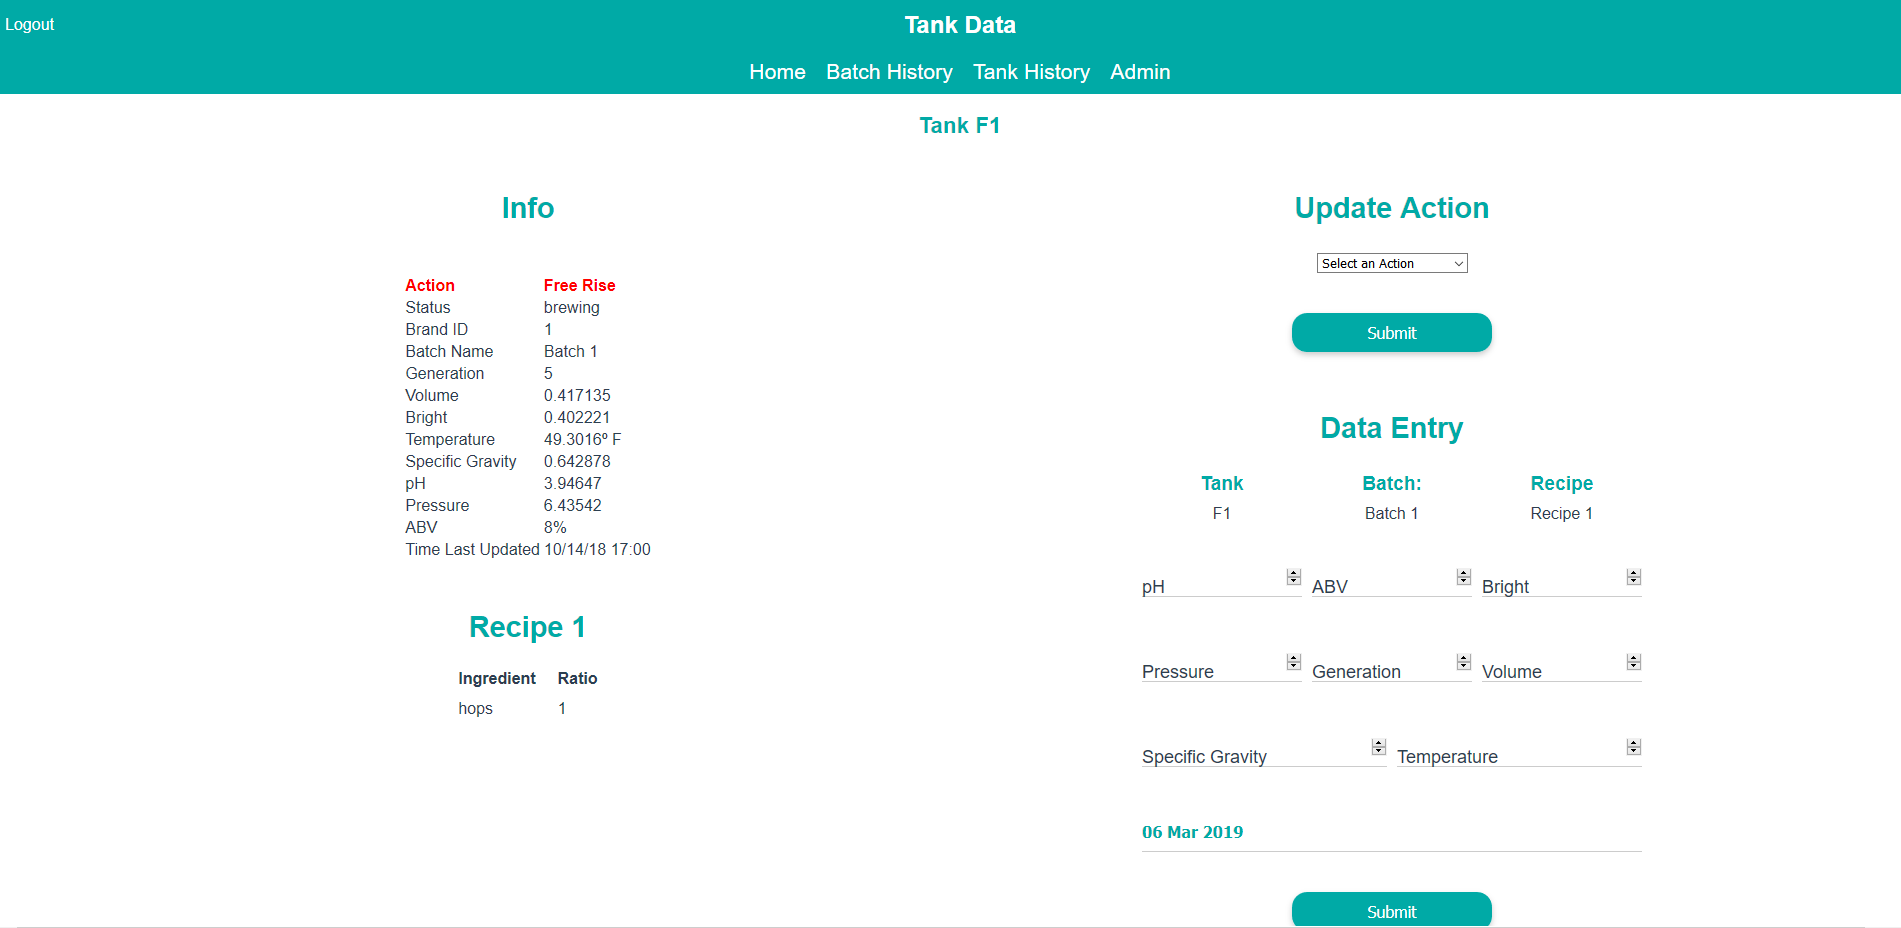
\includegraphics[width=0.9\textwidth]{screenshots/progress_report_screencap-tank_info.png}
    \caption{The new tank info page.}
\end{figure}

\begin{figure}[H]
    \centering
    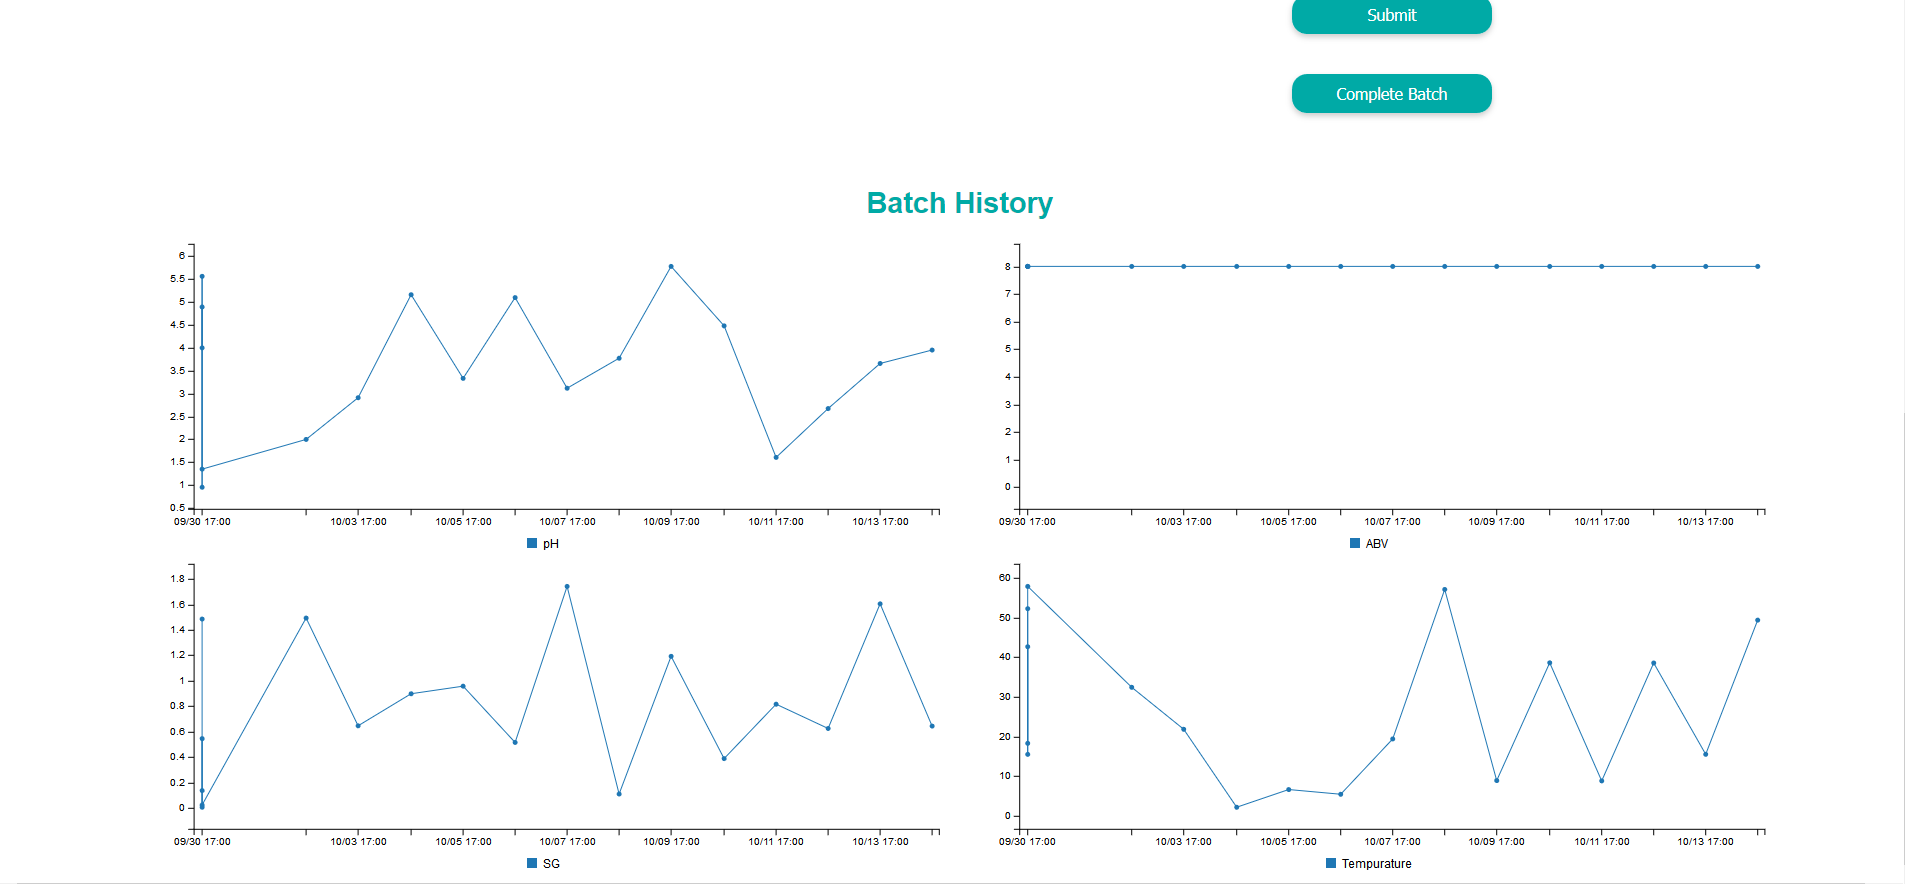
\includegraphics[width=0.9\textwidth]{screenshots/progress_report_screencap-tank_info_charts.png}
    \caption{The charts on the tank info page.}
\end{figure}

\begin{figure}[H]
    \centering
    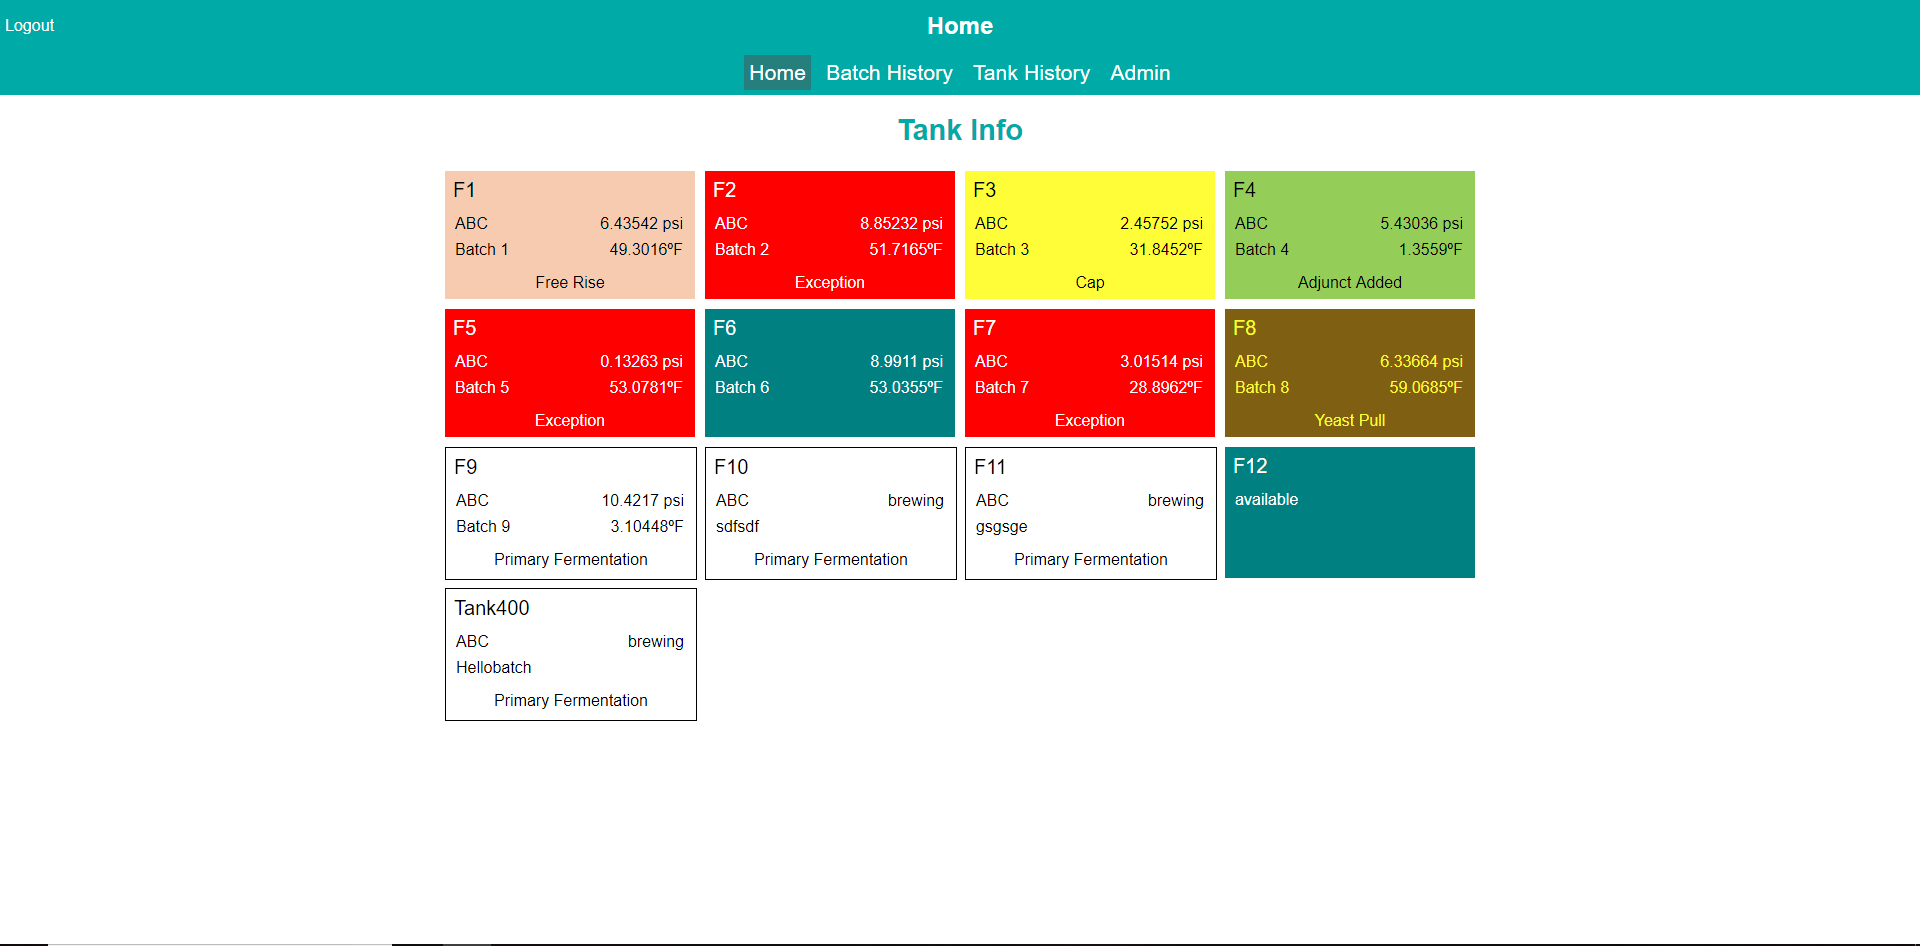
\includegraphics[width=0.9\textwidth]{screenshots/progress_report_screencap-tank_monitoring.png}
    \caption{Color coded tank monitoring by current action.}
\end{figure}

\begin{figure}[H]
    \centering
    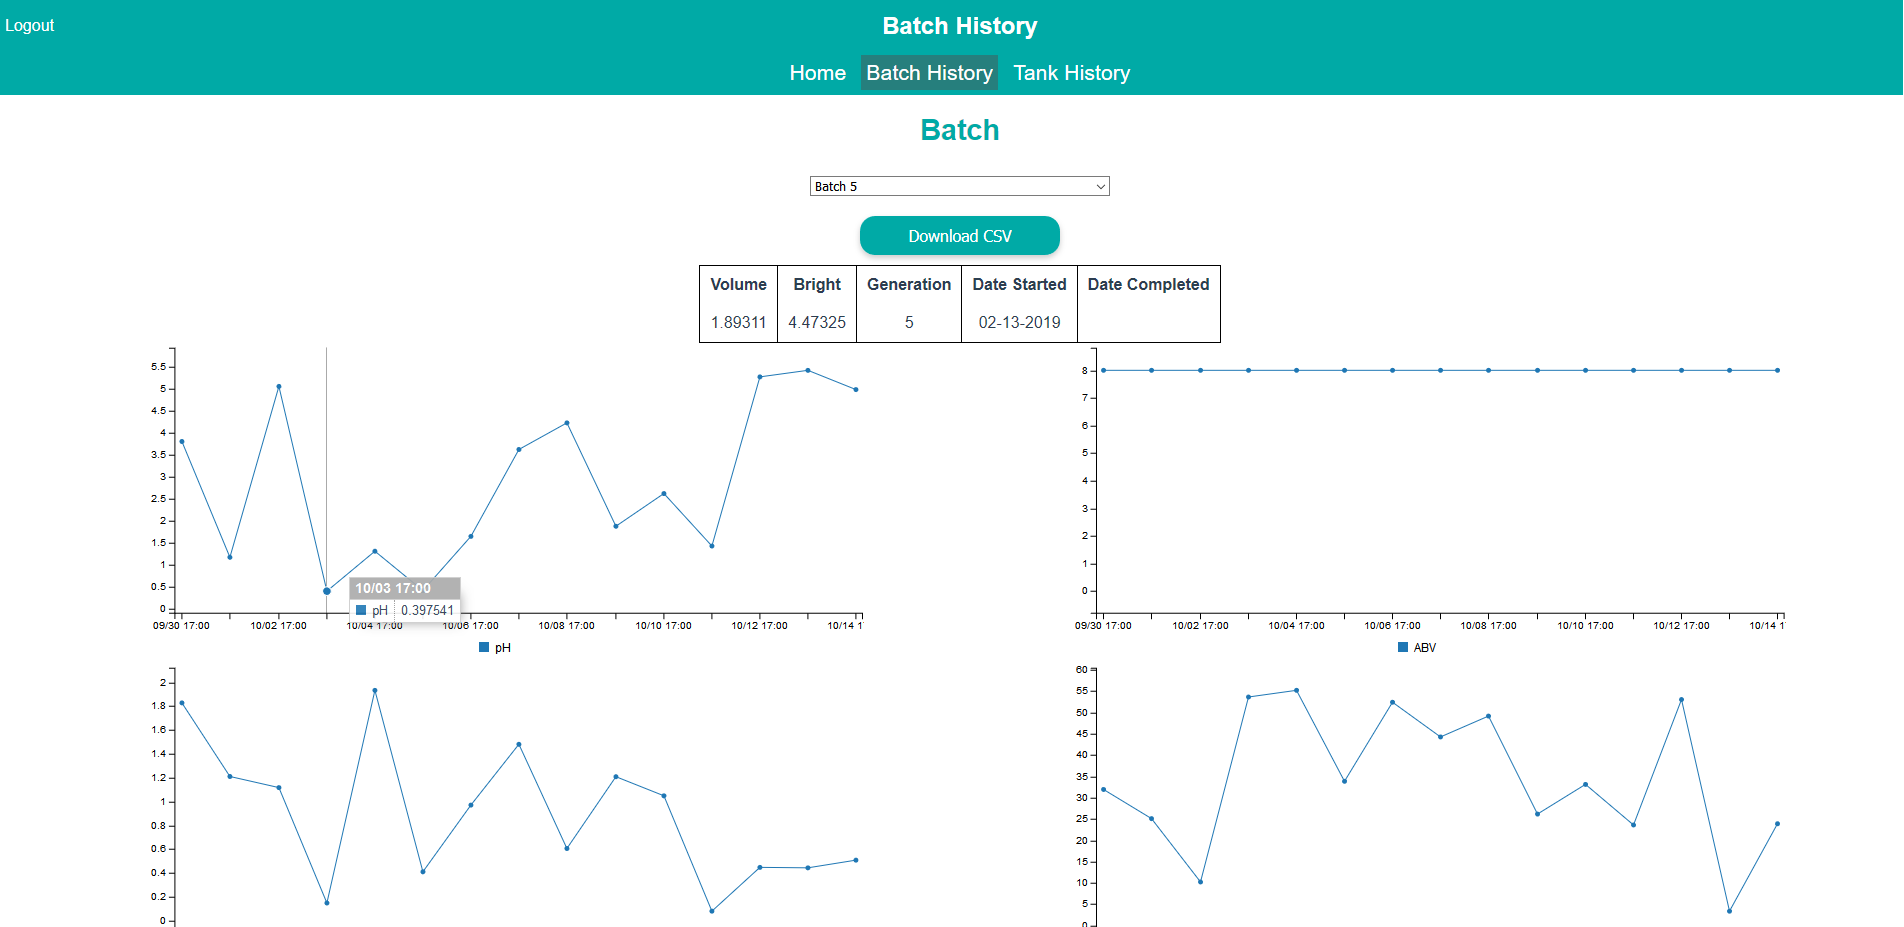
\includegraphics[width=0.9\textwidth]{screenshots/progress_report_screencap-batch_history_1.png}
    \caption{Updated batch history page (top).}
\end{figure}

\begin{figure}[H]
    \centering
    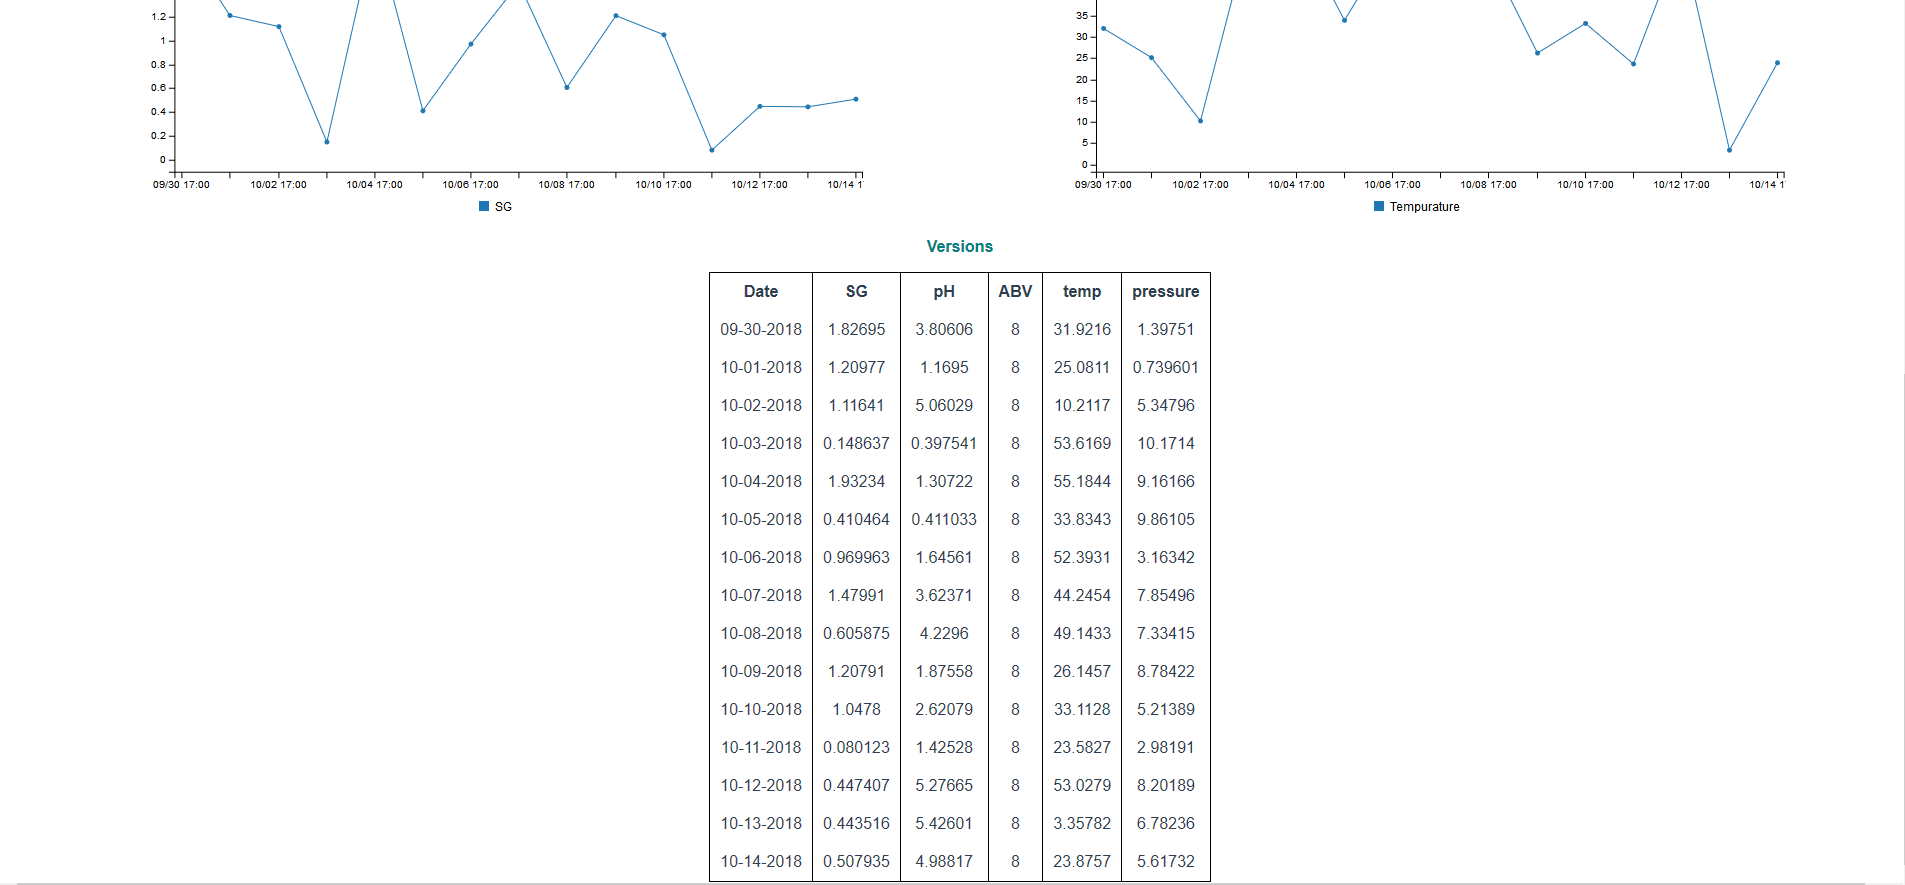
\includegraphics[width=0.9\textwidth]{screenshots/progress_report_screencap-batch_history_2.png}
    \caption{Updated batch history page (bottom).}
\end{figure}

\begin{figure}[H]
    \centering
    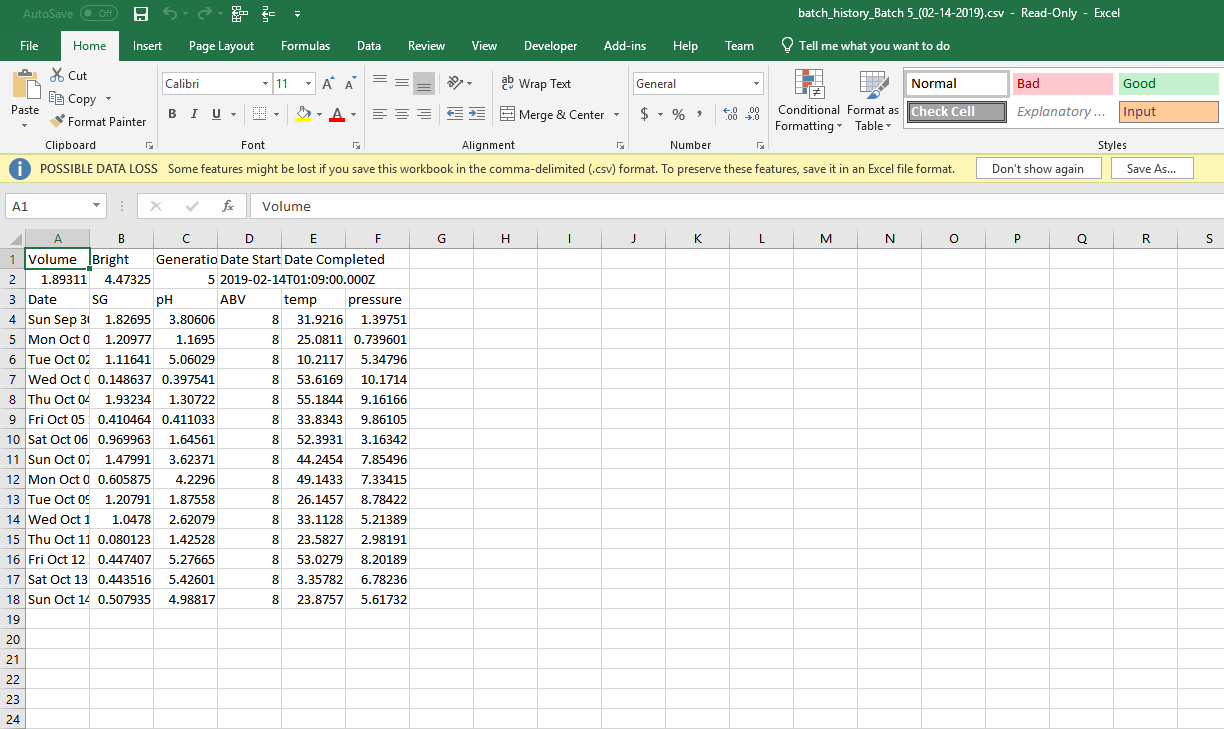
\includegraphics[width=0.9\textwidth]{screenshots/progress_report_screencap-batch_history_csv.png}
    \caption{New batch history page CSV export.}
\end{figure}

\begin{figure}[H]
    \centering
    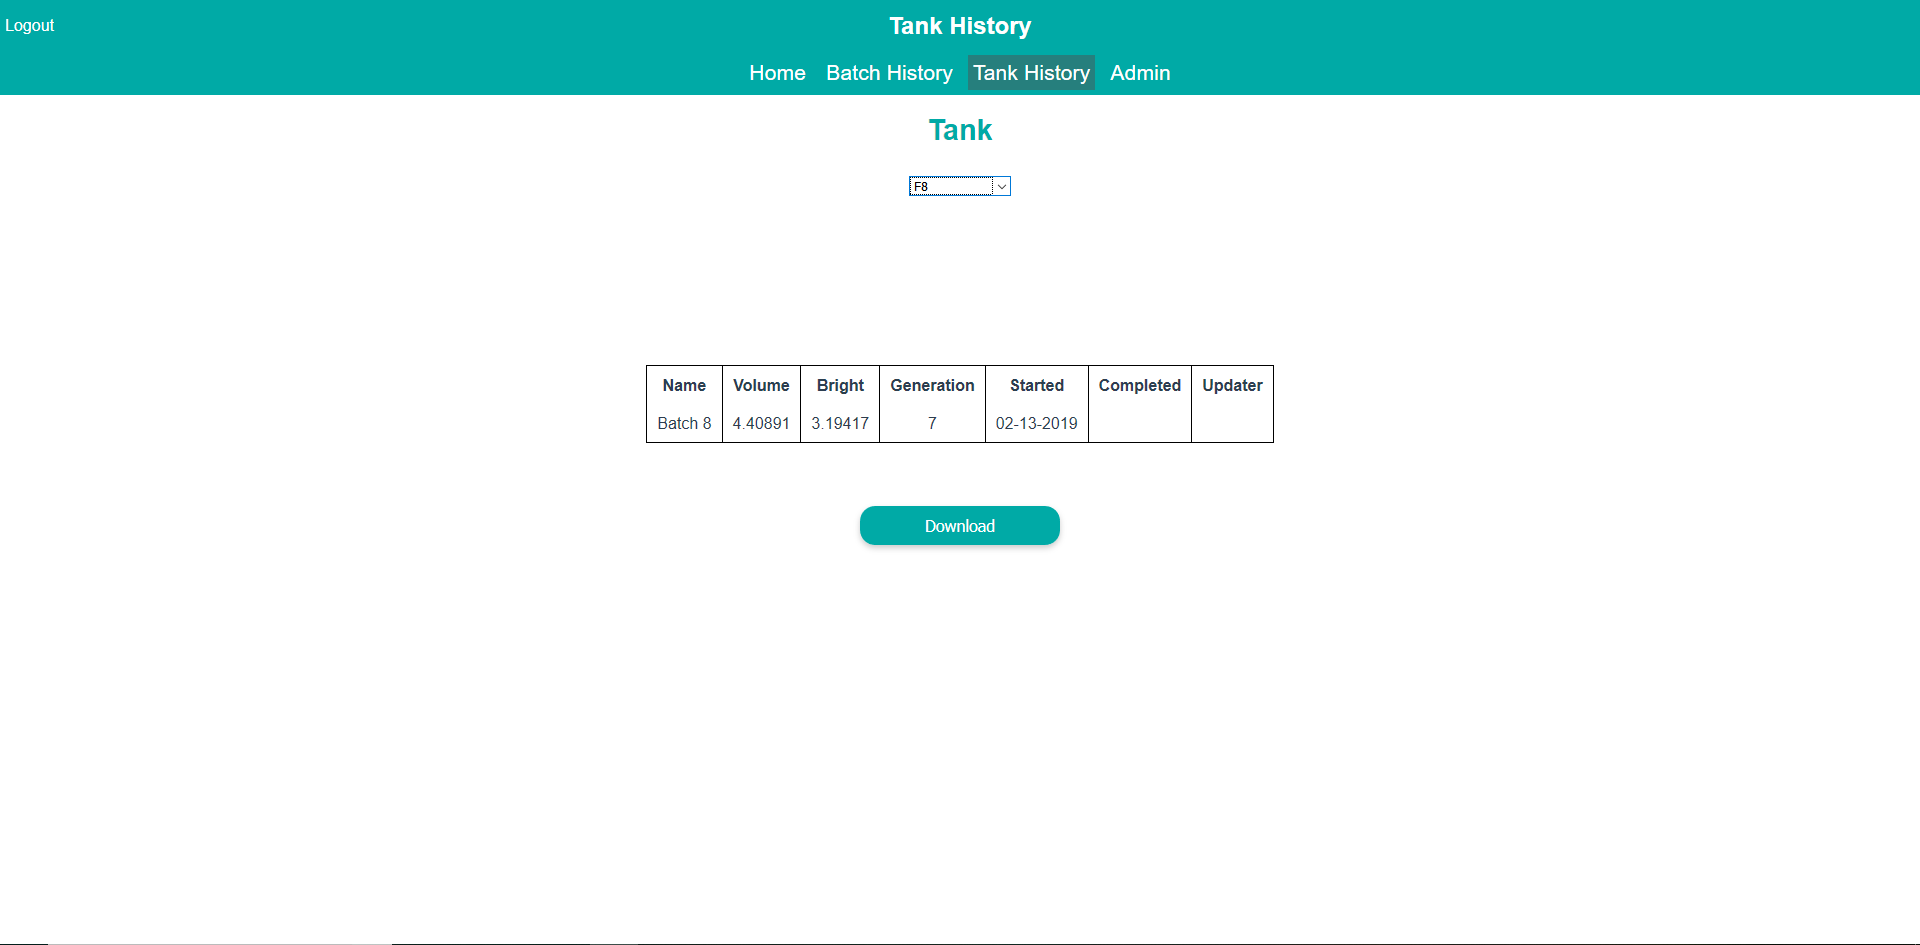
\includegraphics[width=0.9\textwidth]{screenshots/progress_report_screencap-tank_history.png}
    \caption{Updated tank history page.}
\end{figure}

\begin{figure}[H]
    \centering
    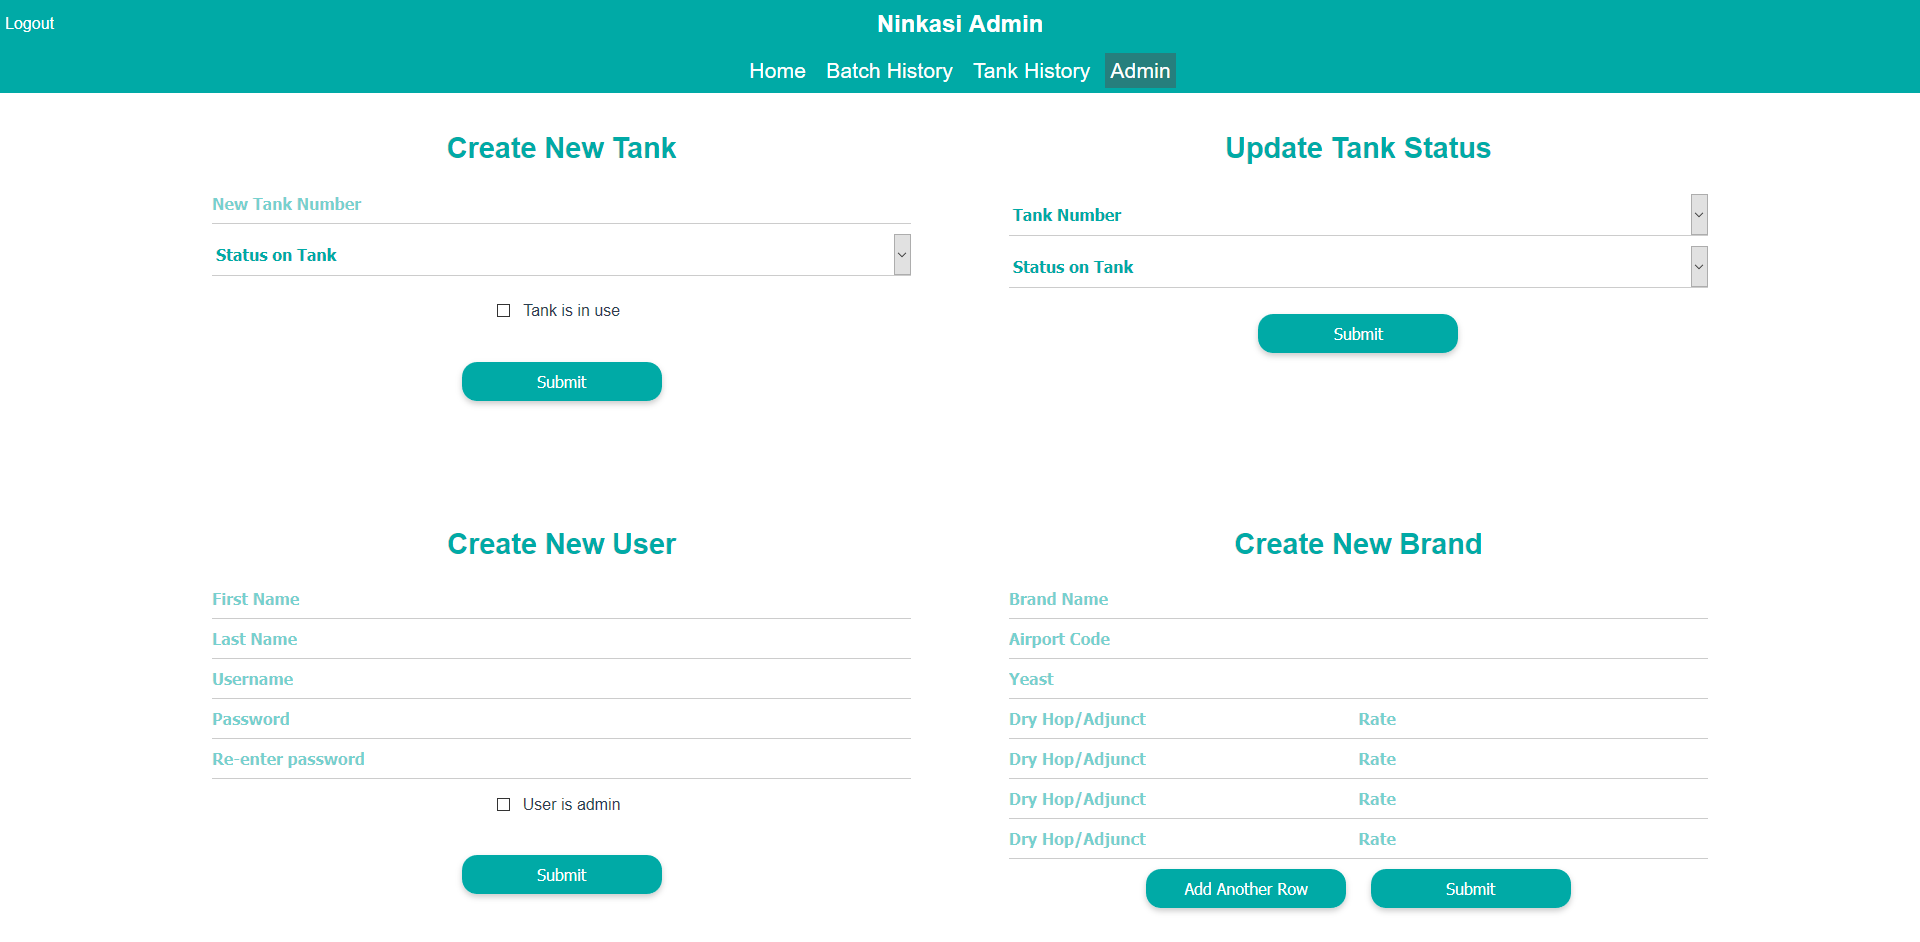
\includegraphics[width=0.9\textwidth]{screenshots/progress_report_screencap-admin_page.png}
    \caption{Admin page.}
\end{figure}

\begin{figure}[H]
    \centering
    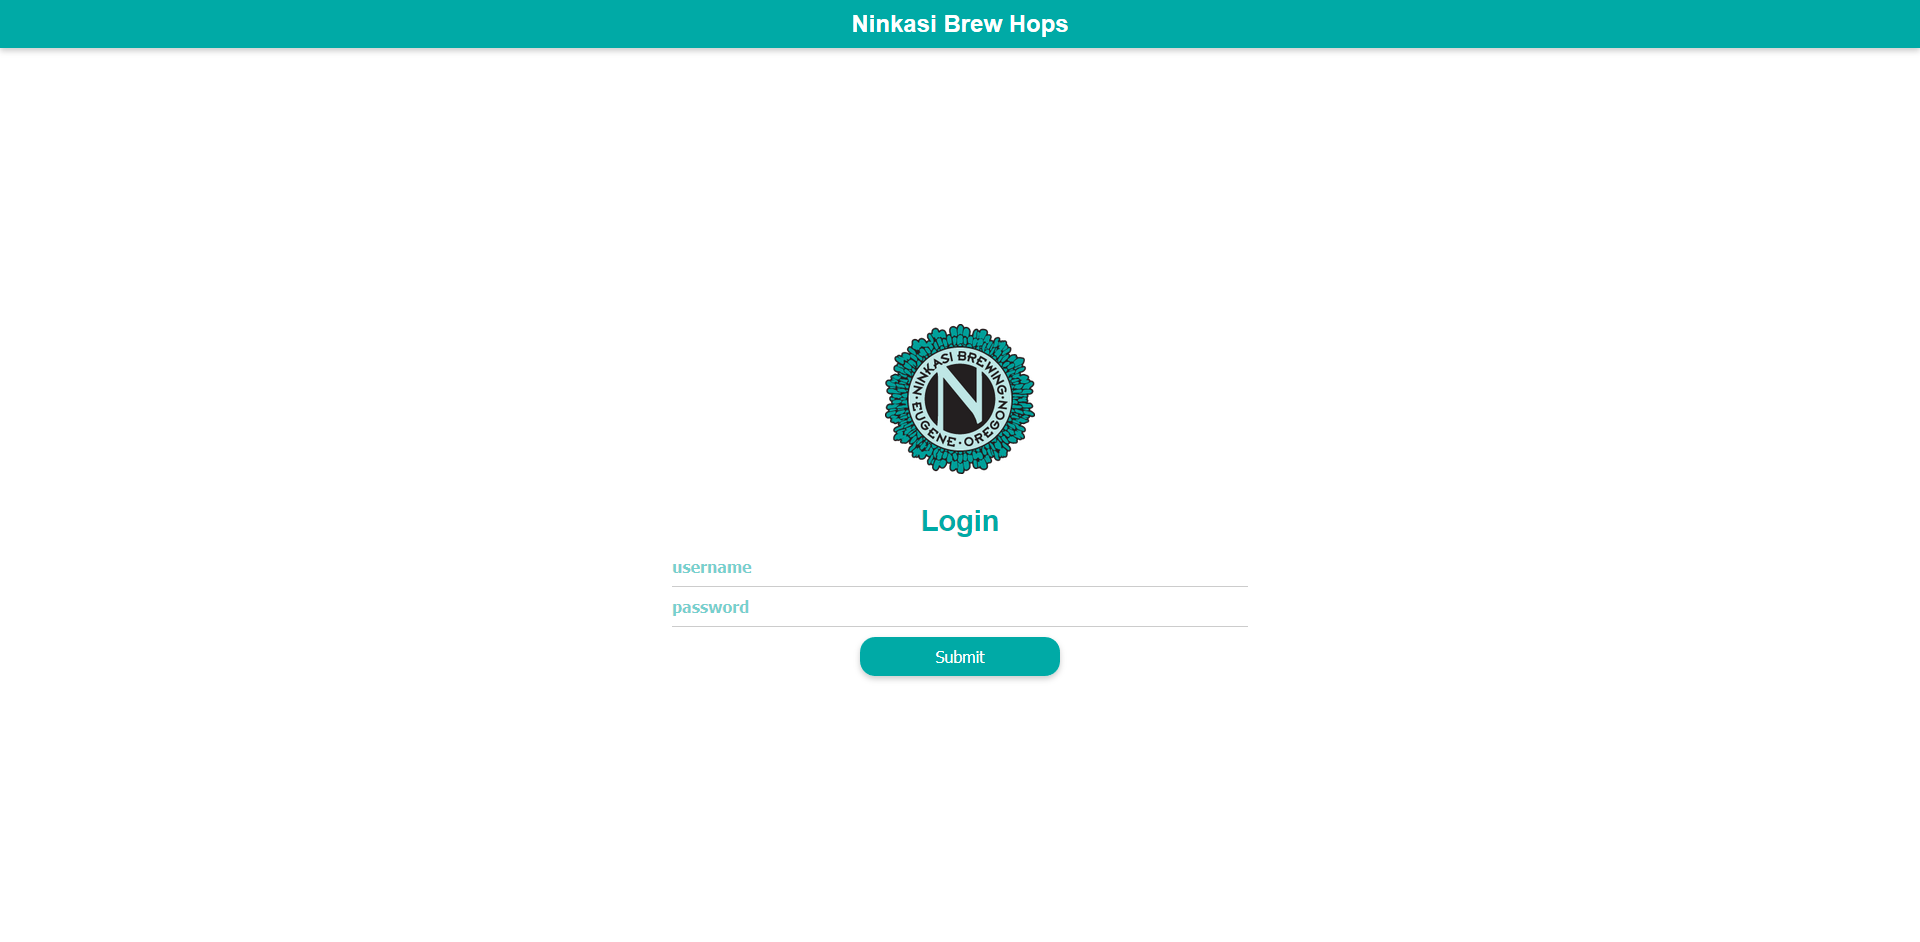
\includegraphics[width=0.9\textwidth]{screenshots/progress_report_screencap-login_page.png}
    \caption{Improved login page.}
\end{figure}

\begin{figure}[H]
    \centering
    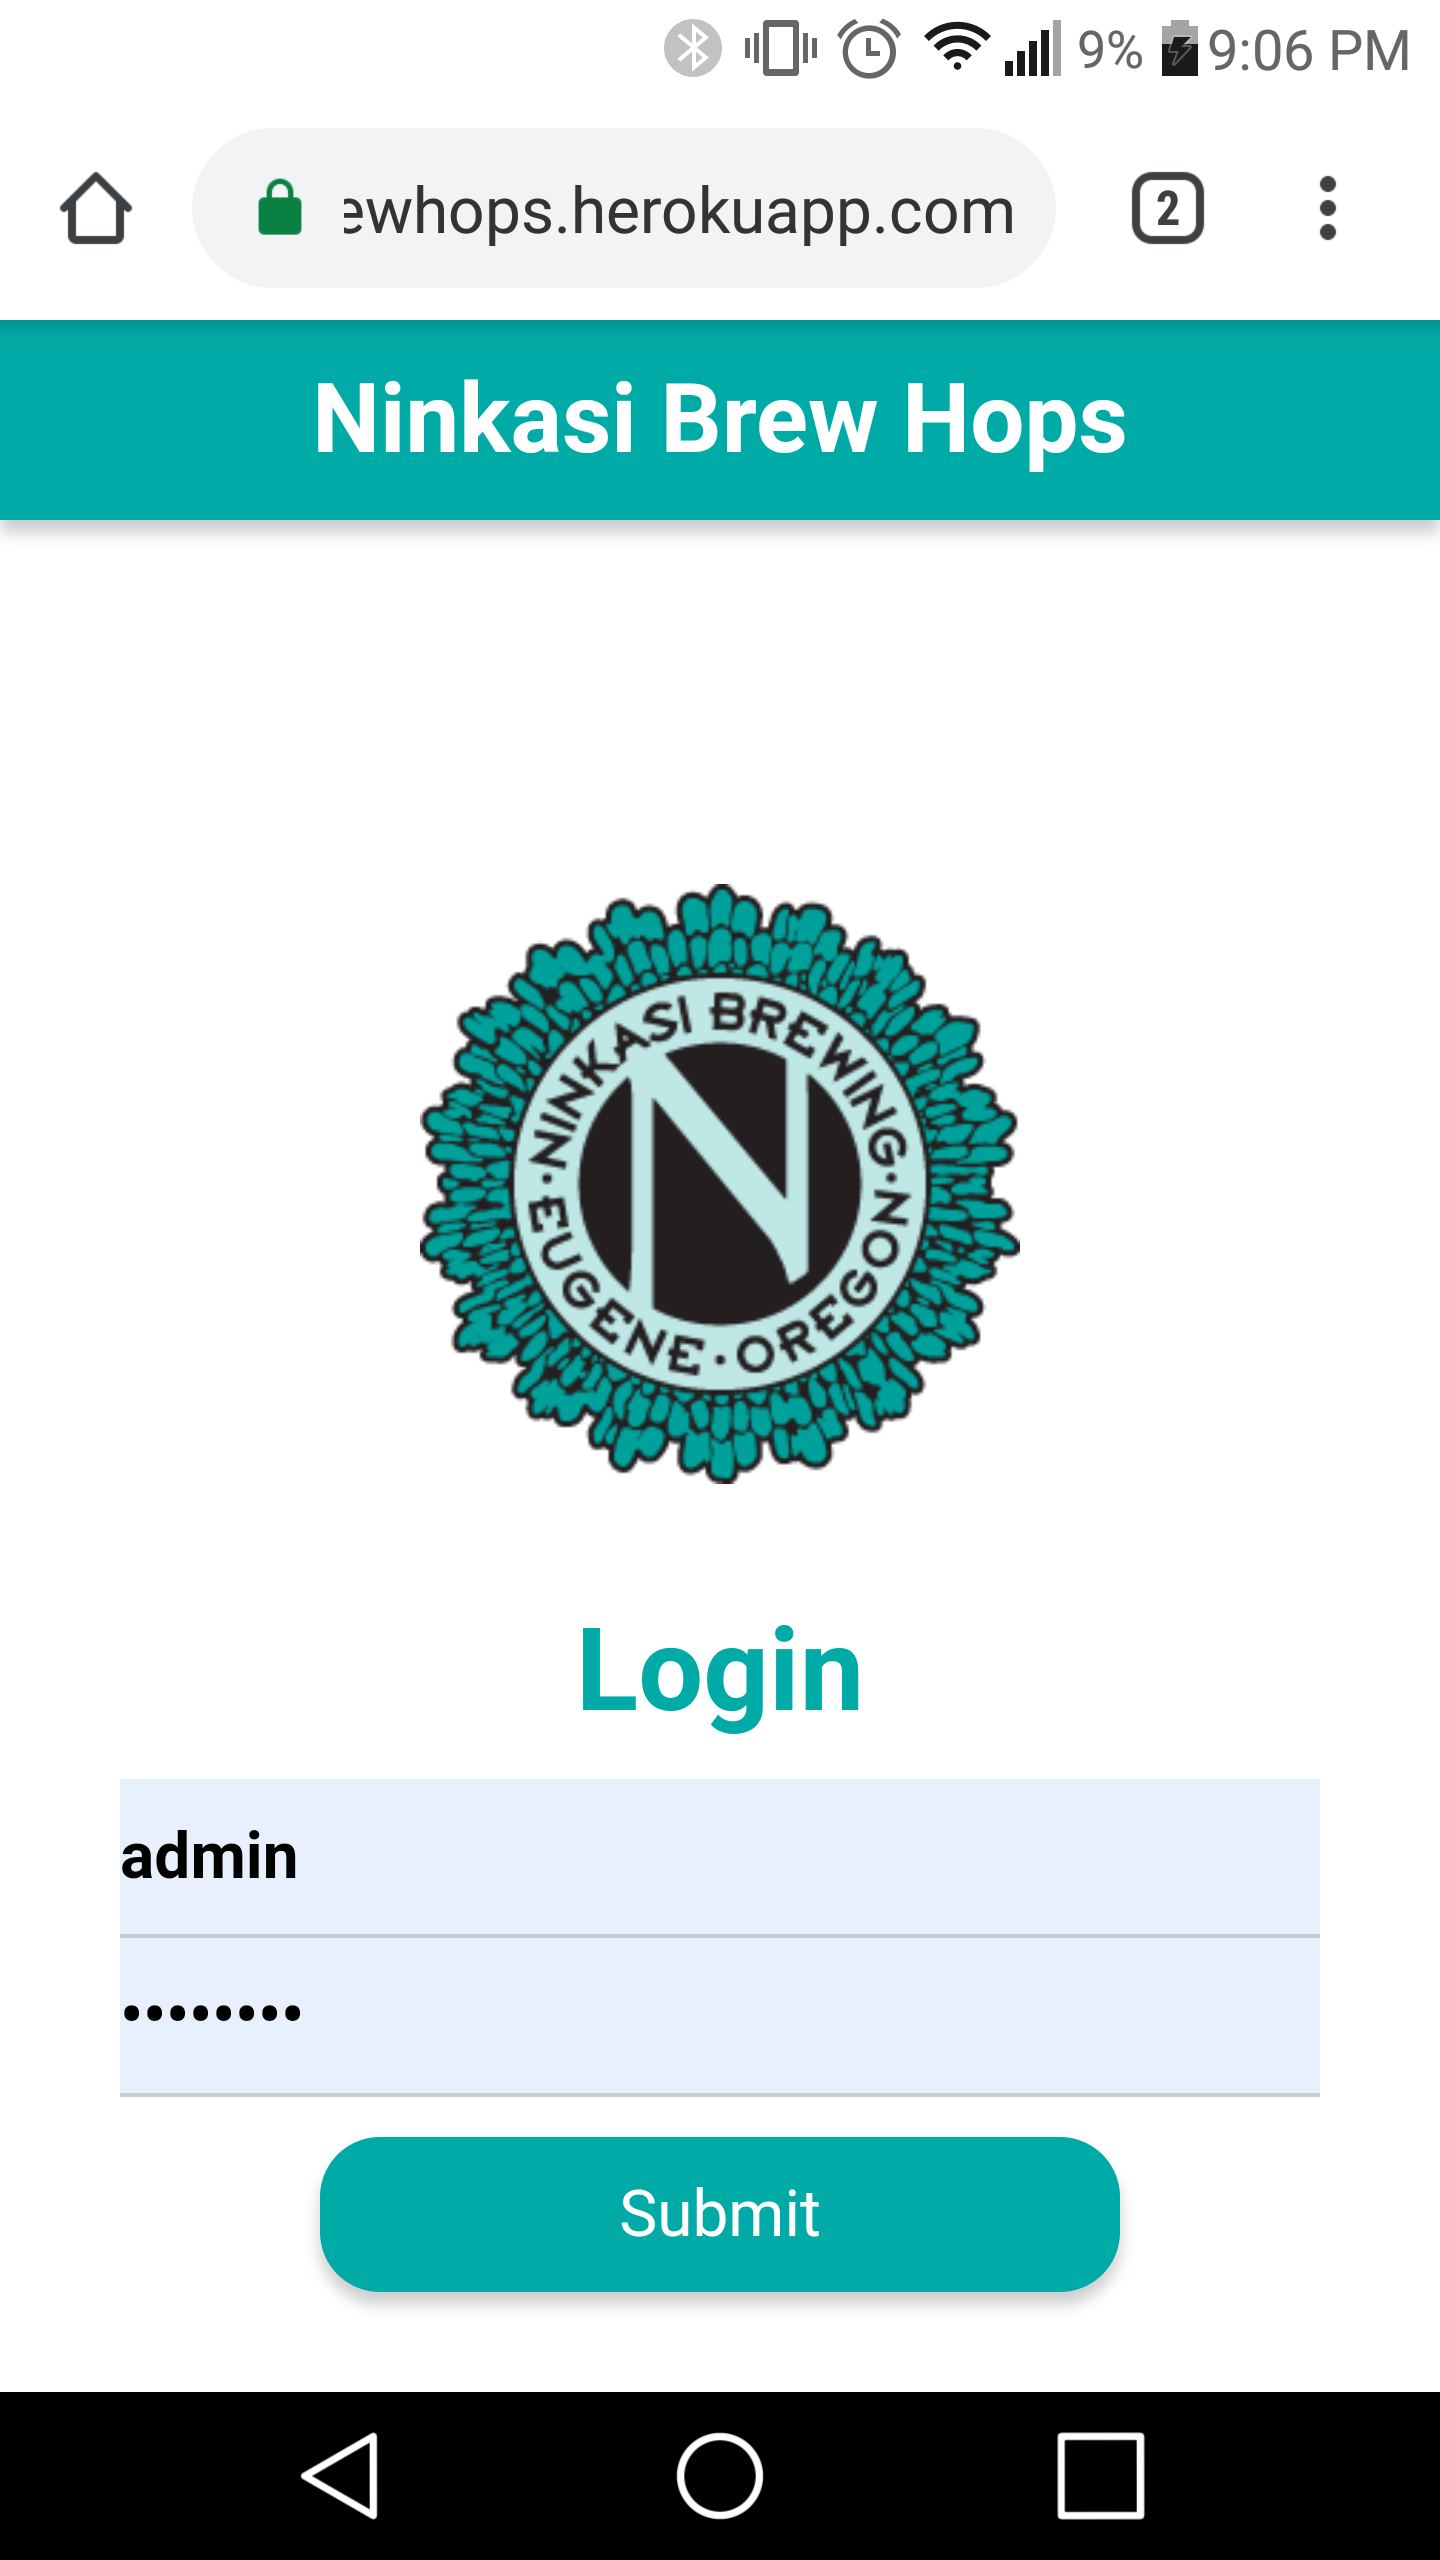
\includegraphics[height=0.4\textheight]{screenshots/progress_report_screencap-mobile_login.png}
    \caption{Mobile login page.}
\end{figure}

\begin{figure}[H]
    \centering
    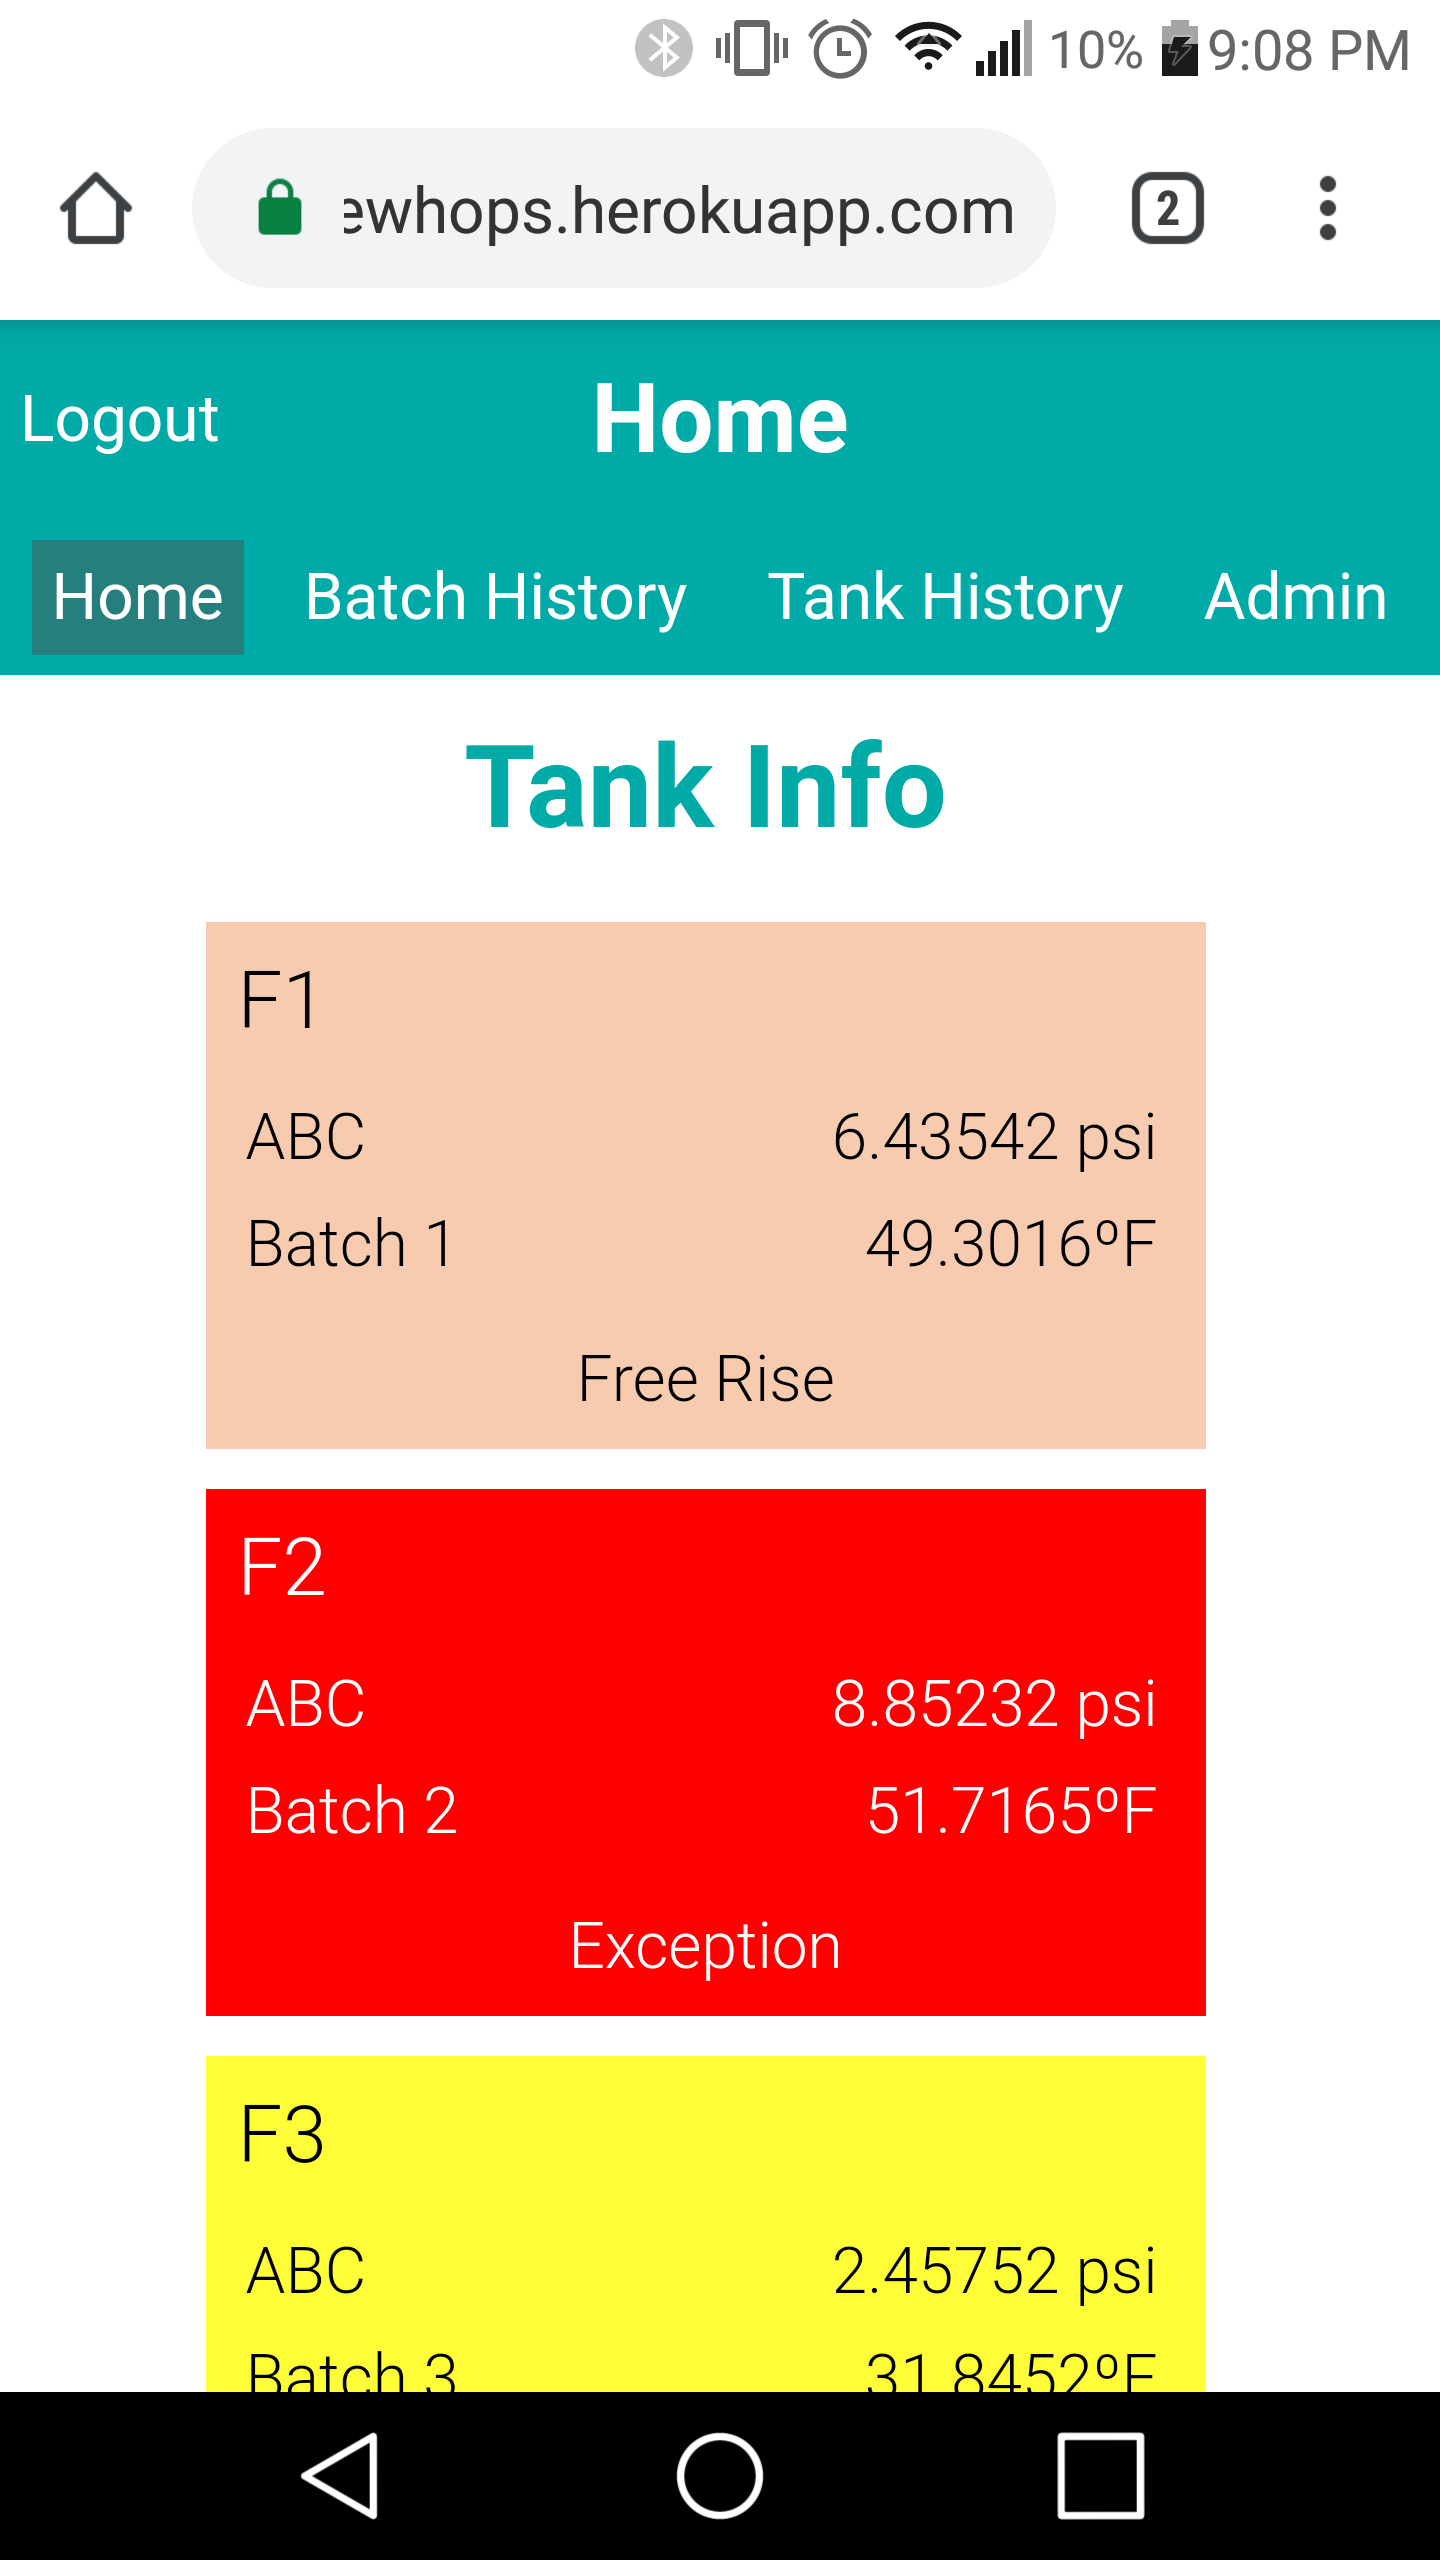
\includegraphics[height=0.4\textheight]{screenshots/progress_report_screencap-mobile_tank_monitoring.png}
    \caption{Mobile tank monitoring page.}
\end{figure}

\begin{figure}[H]
    \centering
    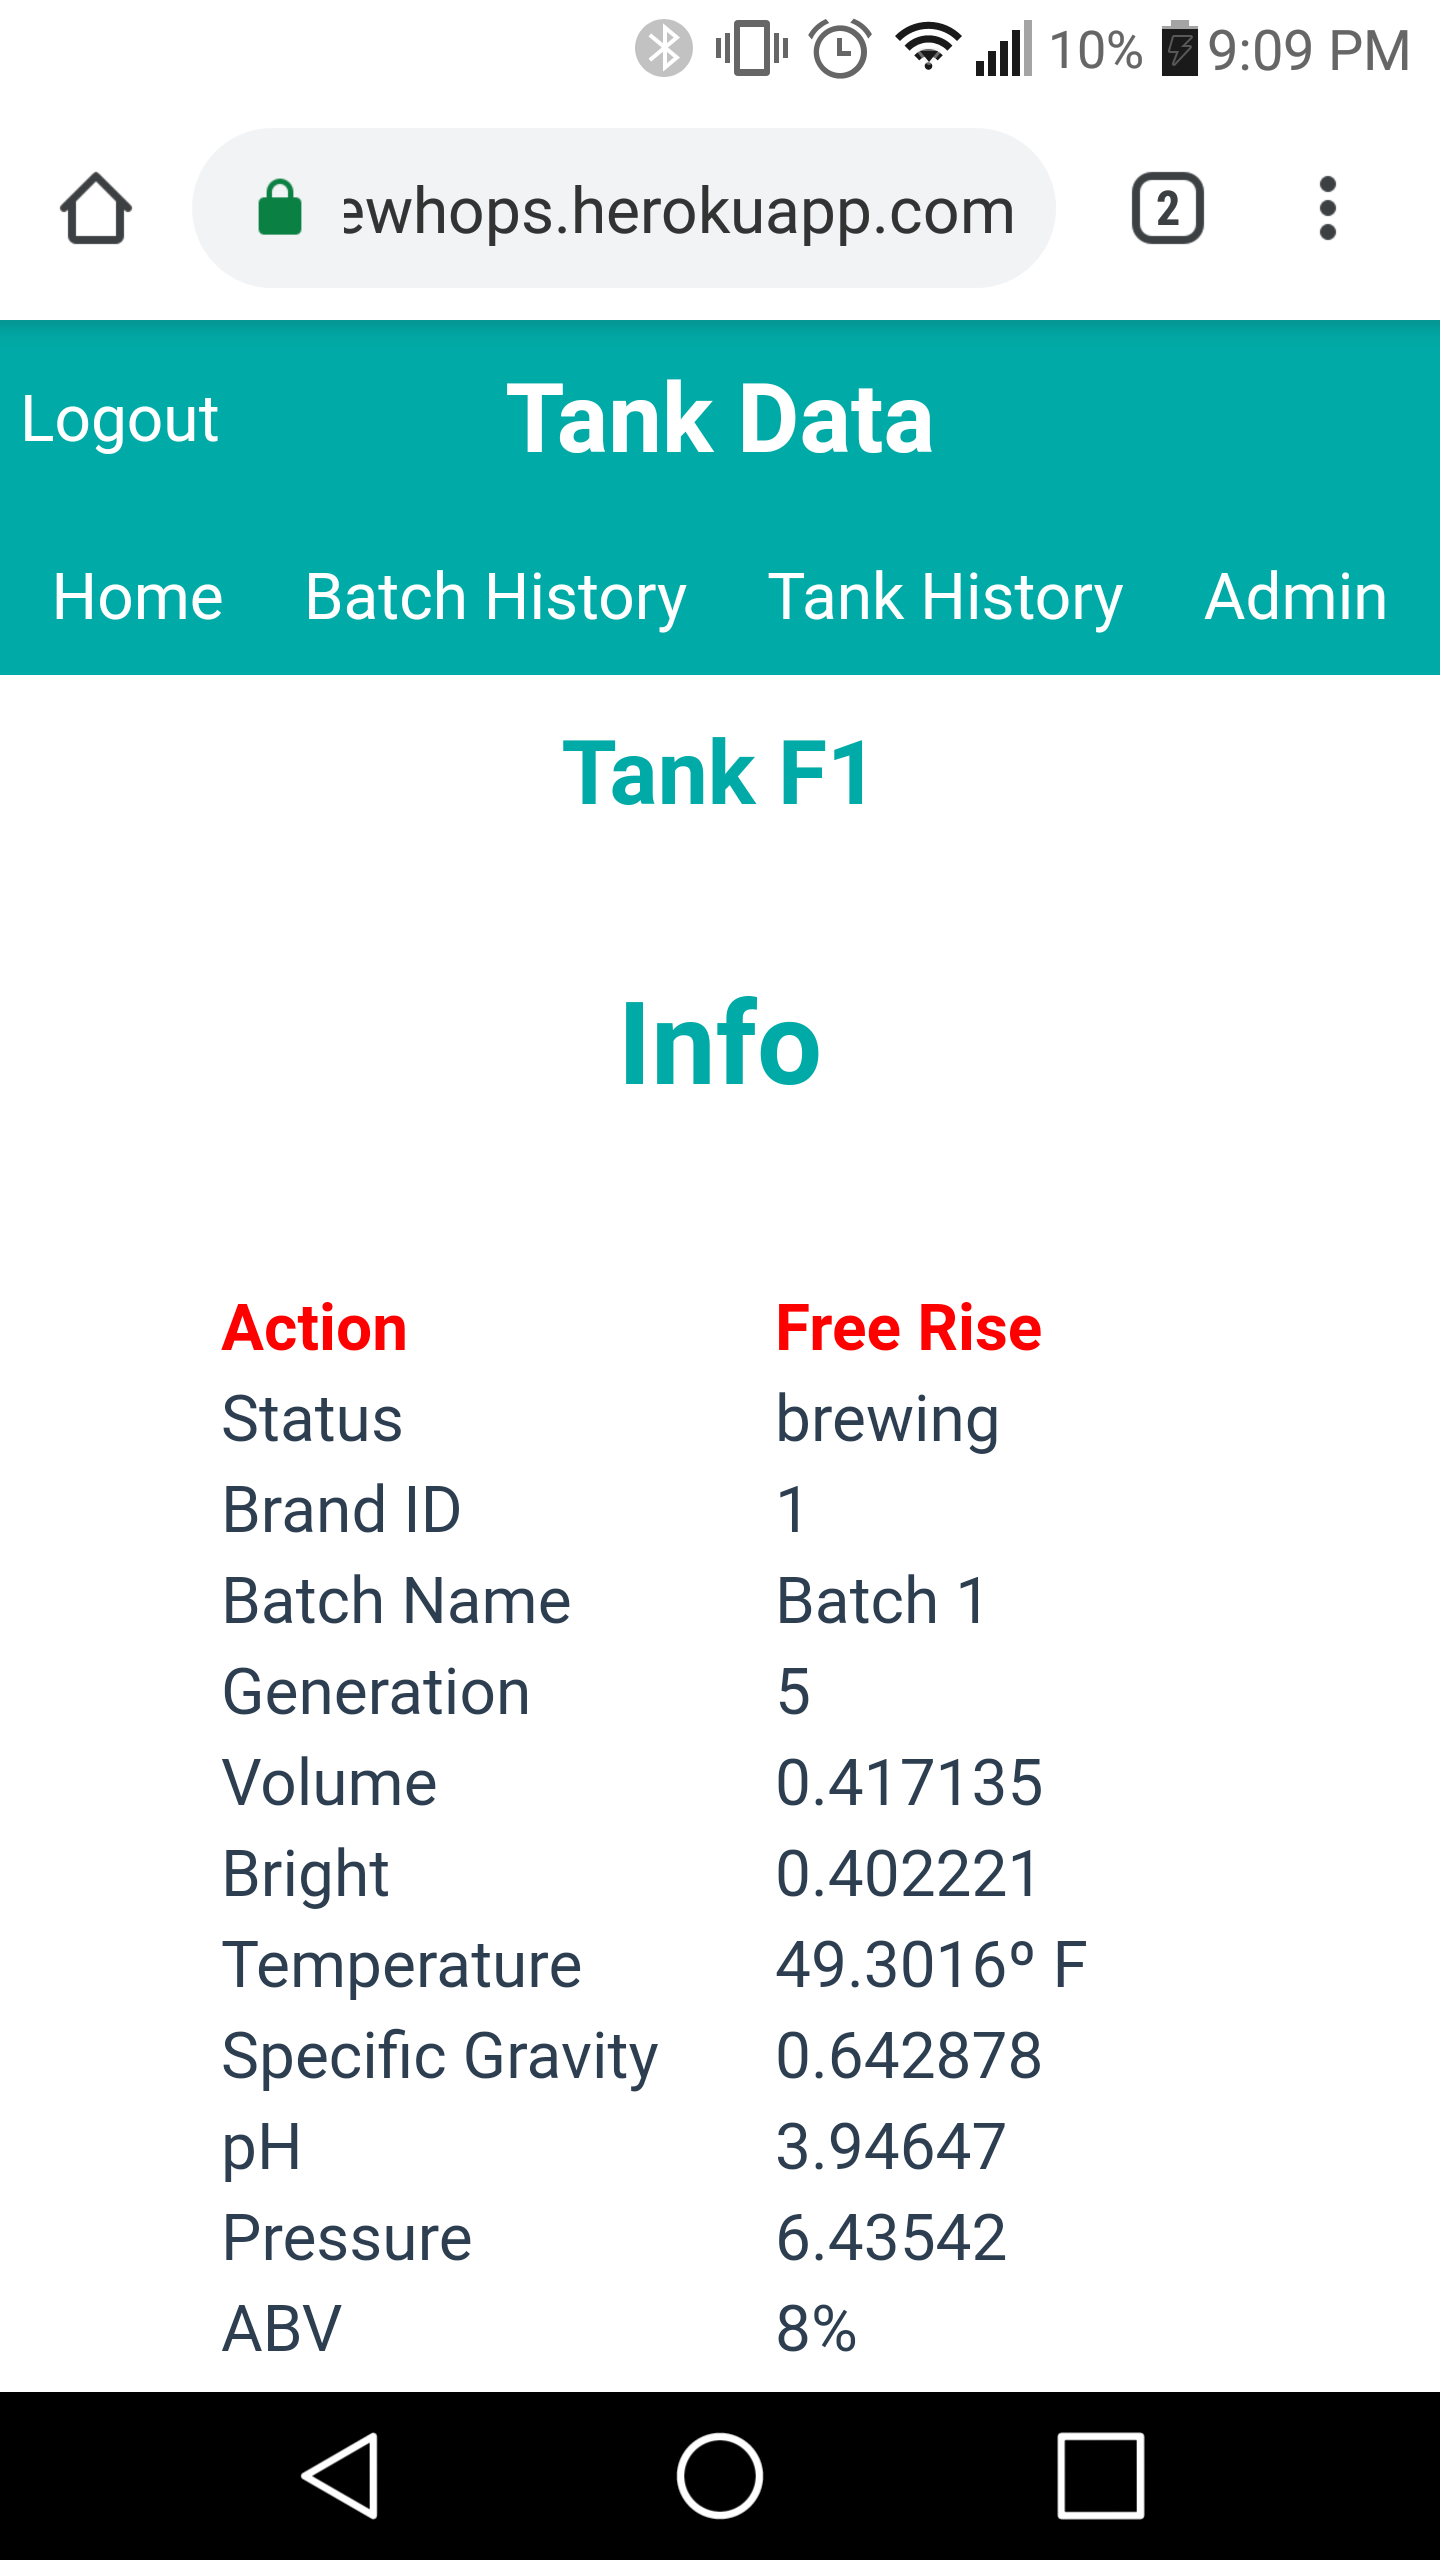
\includegraphics[height=0.4\textheight]{screenshots/progress_report_screencap-mobile_tank_info.png}
    \caption{Mobile tank info page.}
\end{figure}

\begin{figure}[H]
    \centering
    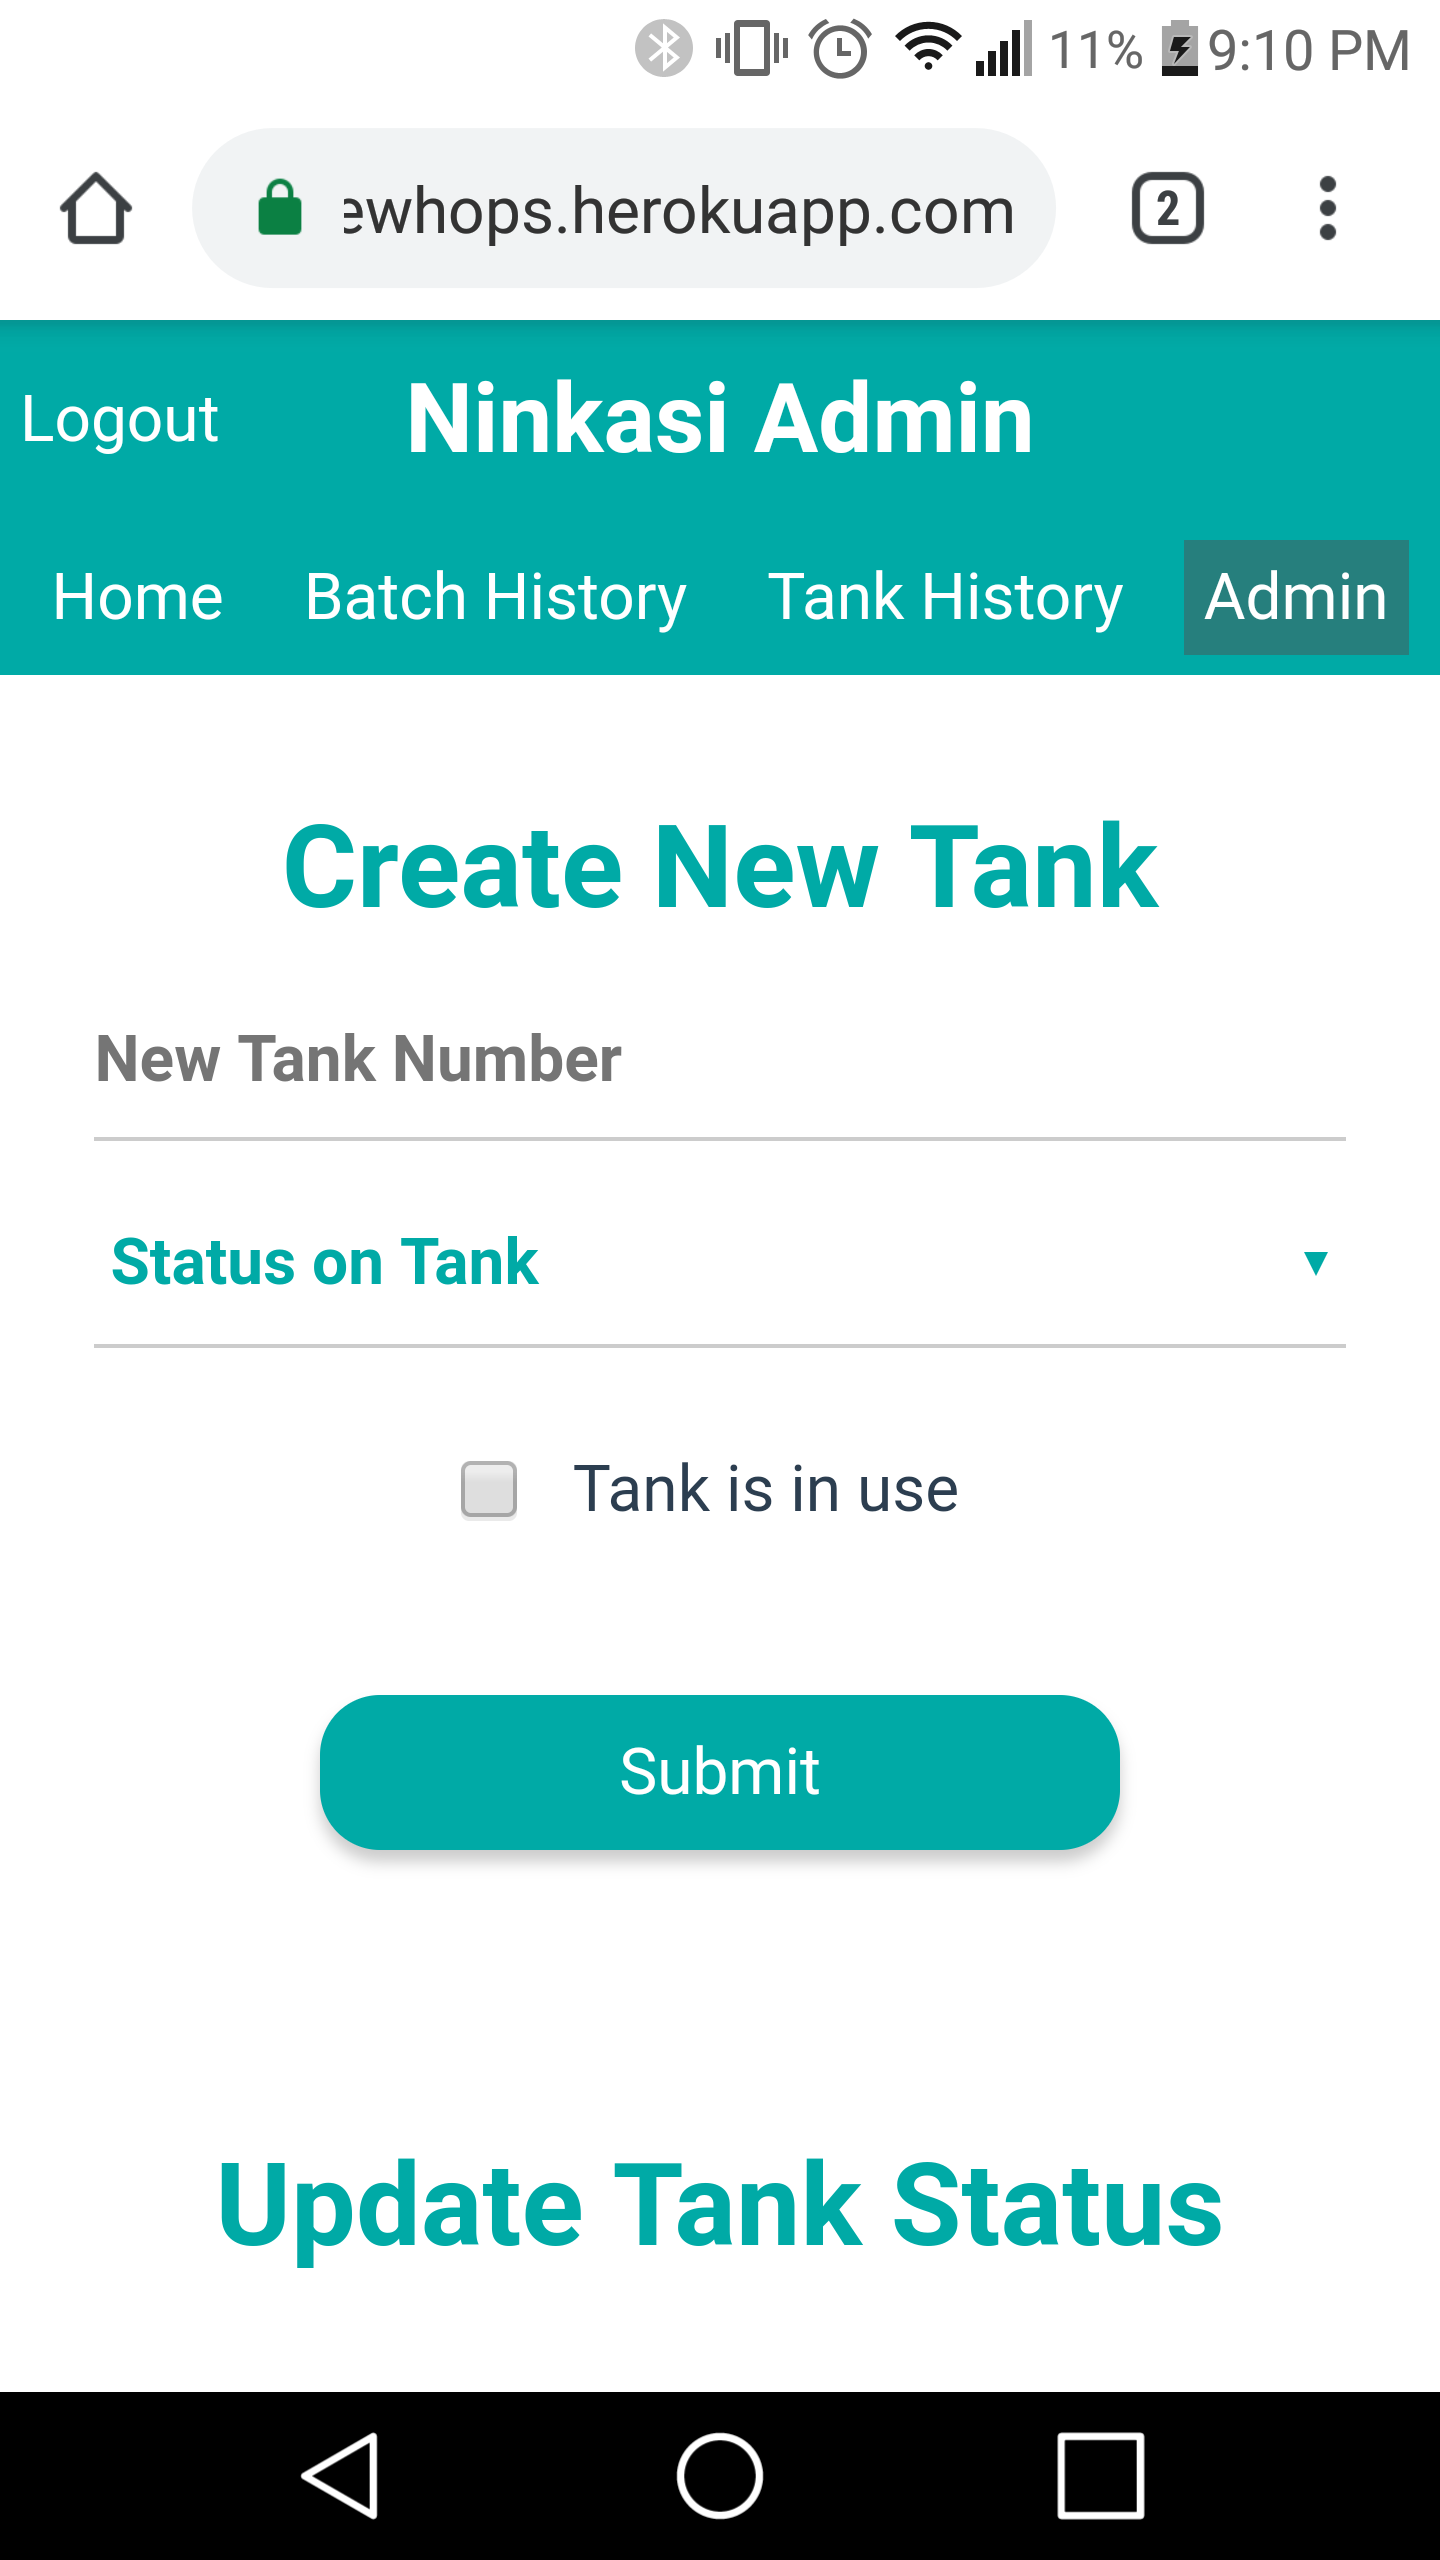
\includegraphics[height=0.4\textheight]{screenshots/progress_report_screencap-mobile_admin.png}
    \caption{Mobile admin page.}
\end{figure}

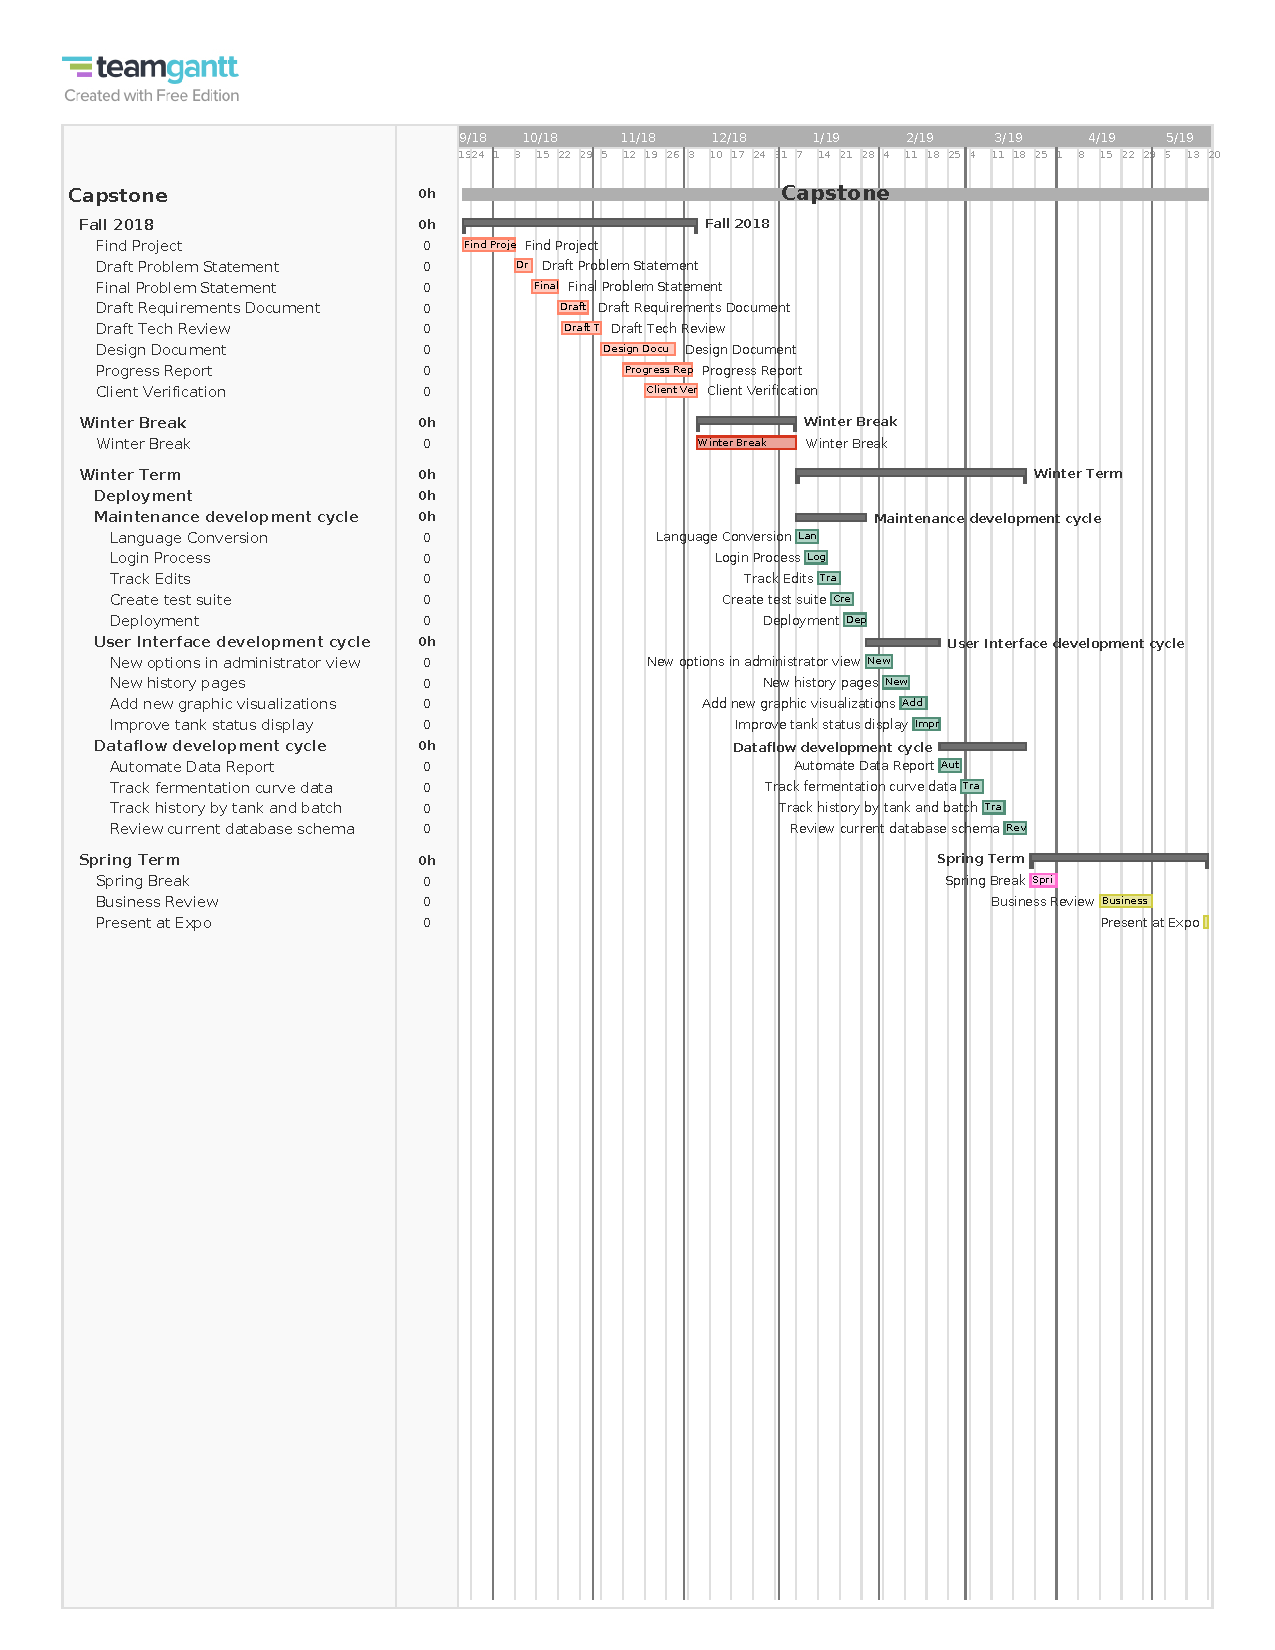
\includepdf[pages=1]{Capstone.pdf}

\end{document}
